\documentclass{report}
\usepackage[utf8]{inputenc}
\usepackage{amsmath}
\usepackage{graphicx}
\usepackage{hyperref}
\parindent=0pt
\usepackage[a4paper, total={165mm, 235mm}]{geometry}
\usepackage[section]{placeins}
\usepackage{enumitem}
\usepackage{caption}
\usepackage{parskip}
\usepackage{multirow}
\usepackage{biblatex}
\addbibresource{Bibliography.bib}
\usepackage{wrapfig}

\title{PySPI for Persistent Sources}
\author{Möller, Julius}
\date{June 2023}

\begin{document}

\begin{titlepage}
    
    
\includegraphics[height=1cm]{Images/General/MPE_logo_189x180px.jpg}
    \hfill
    
\includegraphics[height=1cm]{Images/General/PH.pdf}
    
\includegraphics[height=1cm]{Images/General/tumlogo.pdf}

    \begin{center}
        \vspace{1cm}
        \large

        Max Planck Institute for Extraterrestrial Physics
        

        \vspace{1.5cm}
        \large
        Thesis for Master of Science in Astrophysics
        
        \vspace{3cm}
        \Huge
        PySpi for Persistent Sources
        
        \vspace{3cm}
        
        \LARGE
        Julius Möller
        
        \vspace{1.5cm}
        \large
        June 2023
        
        
        \vspace{6.5cm}
        
        
        
        \large
        Technische Universität München

        Fakultät für Physik
        
        
        
    \end{center}
\end{titlepage}


\tableofcontents

\pagebreak

\chapter{Introduction}
\label{Introduction}
\section{About INTEGRAL}


\begin{wrapfigure}{r}{0.50\textwidth}
  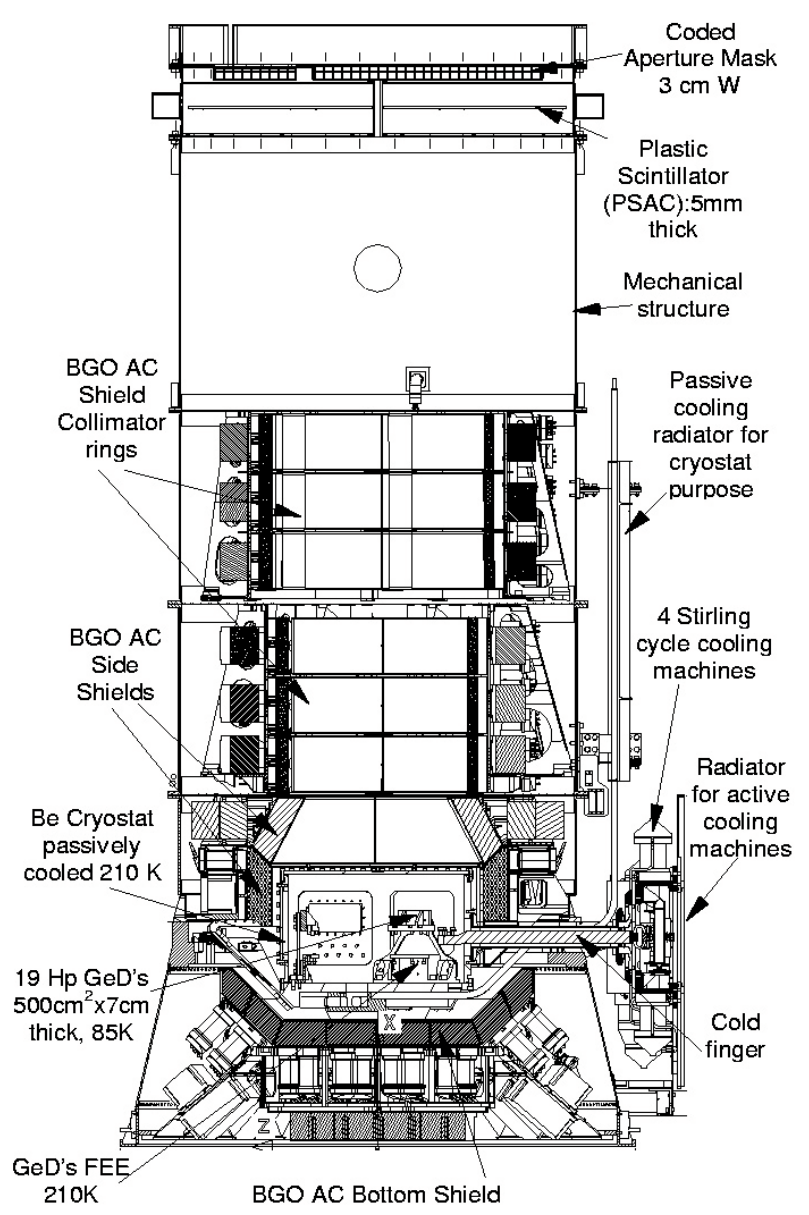
\includegraphics[width=\linewidth]{Images/General/SPI_cut_view_verdenne_2003.PNG}
  \vspace{-20pt}
  \caption{Cut-out view of the SPI spectrometer \cite{refId0}.}
  \vspace{-20pt}
  \label{SPI cut view}
\end{wrapfigure}


The INTErnational Gamma-Ray Astrophysics Laboratory (INTEGRAL) is an ESA space telescope with contributions from NASA and the RKA. Its mission began on October 17, 2002, when a Proton-DM2 rocket launched it from the Russian Baikonur spaceport in Kazakhstan into a 3-day, highly elliptical orbit with an apogee of 153000km and a perigee of 9000km, although this has not remained constant over the course of its lifetime. This places INTEGRAL mostly above radiation belts that would cause high instrumental backgrounds from charged-particle activation, and is why data collecting is halted during hours of close Earth-proximity. Initially, INTEGRAL had a 2+3-year planned lifetime, which it has greatly exceeded due to its lower than expected fuel consumption. Since then, its science operations have been repeatedly extended, currently up to the end of 2024, with some difficulties along the way such as its failed thrusters in July 2020 (compensated through the use of reaction wheels) and an uncontrolled tumbling caused by a single event upset in September 2021. The satellite is predicted to reenter Earth's atmosphere in 2029.



Onboard INTEGRAL are two main instruments: the Imager on-Board the INTEGRAL Satellite (IBIS) and the SPectrometer of INTEGRAL (SPI). IBIS specializes in being able to locate sources effectively. With an angular resolution of 12 arcmin, it can locate bright sources with arcmin precision in its $9^\circ \times 9^\circ$ field of view, and covers an energy range from 15keV to 10MeV. 

\subsection{About SPI}




SPI, the instrument used in this thesis and illustrated in figure \ref{SPI cut view}, specializes in its detailed energy resolution. At 1.3MeV, it is able to resolve energies with 2.5keV precision. It has a field of view of $16^\circ$ and an energy range covering 20keV to 8MeV. One decisive advantage SPI has in comparison to many comparable instruments is that its response matrices are based on extensive ground calibrations and Monte-Carlo simulations, as opposed to relying on astronomical sources such as the Crab Nebula.





\subsubsection*{Detectors}
SPIs detectors are composed of an hexagonal array of 19 reverse-electrode n-type germanium detectors. With a mean crystal weight of 951g and mean volume of $178\text{cm}^3$, the total geometrical area for a flux parallel to the axis is $508\text{cm}^2$. Under normal working conditions, a voltage of 4000V is applied to each detector independently, and this voltage is variable between zero and 5000V. 

The germanium detectors require temperatures below 100K to work effectively, preferably as low as 85K in order to slow the effects of radiation damage. To accomplish this, SPI is equipped with an active cryogenic system. The Ge array is fixed on a Be plate, which is placed inside the cryostat. The plate is connected to the Stirling cycle cryocoolers to provide active cooling. 

Despite the low temperatures and hexagonal design to reduce the probability of hole traps in the semiconductor, radiation damage will inevitably accumulate over the course of a year or more. To combat this issue the detectors can undergo an annealing process, in which they are held at a temperature of $105^\circ \text{C}$ over the course of one or two days, depending on the damage. An annealing process of two days is enough to fully recover the energy resolution after radiation damage leading to a 20\% increase in the FWHM at 1.3MeV \cite{refId0}.

Each detector is connected to a preamplifier, which outputs the charge integrated signal (proportional to the measured energy) and the PSD signal (see below) to the detectors respective electronic chains for processing.

\subsubsection*{Pulse Shape Discrimination electronics (PSD)}



In order to suppress background events, SPI is equipped with Pulse Shape Discrimination (PSD) electronics. The idea is that localized beta decays in the detector material, which would otherwise be indistinguishable from photon energy deposits, only interact in a small volume of the detector, resulting in a single current pulse in the preamplifier. Gamma-rays, which primarily deposit energy via multiple compton scatterings in the detector volume, thus lead to a broader signal. 

Each detector is connected to its own PSD electronic system, which is only triggered in a certain energy range. The lower level threshold (LLD) is configurable, and has been varied between 400keV and 750keV over the missions lifetime, where as the upper level threshold (ULD) is fixed at around 8MeV. Naturally, processing and analyzing the shape of a signal takes time, and when another event is measured within this time it is stored without any PSD information. The PSD electronics thus have an efficiency that can be approximated around 85\% \cite{Roques}.



\subsubsection*{Anticoincidence shield (ACS)}

\begin{wrapfigure}{R}{0.30\textwidth}
  \vspace{-20pt}
  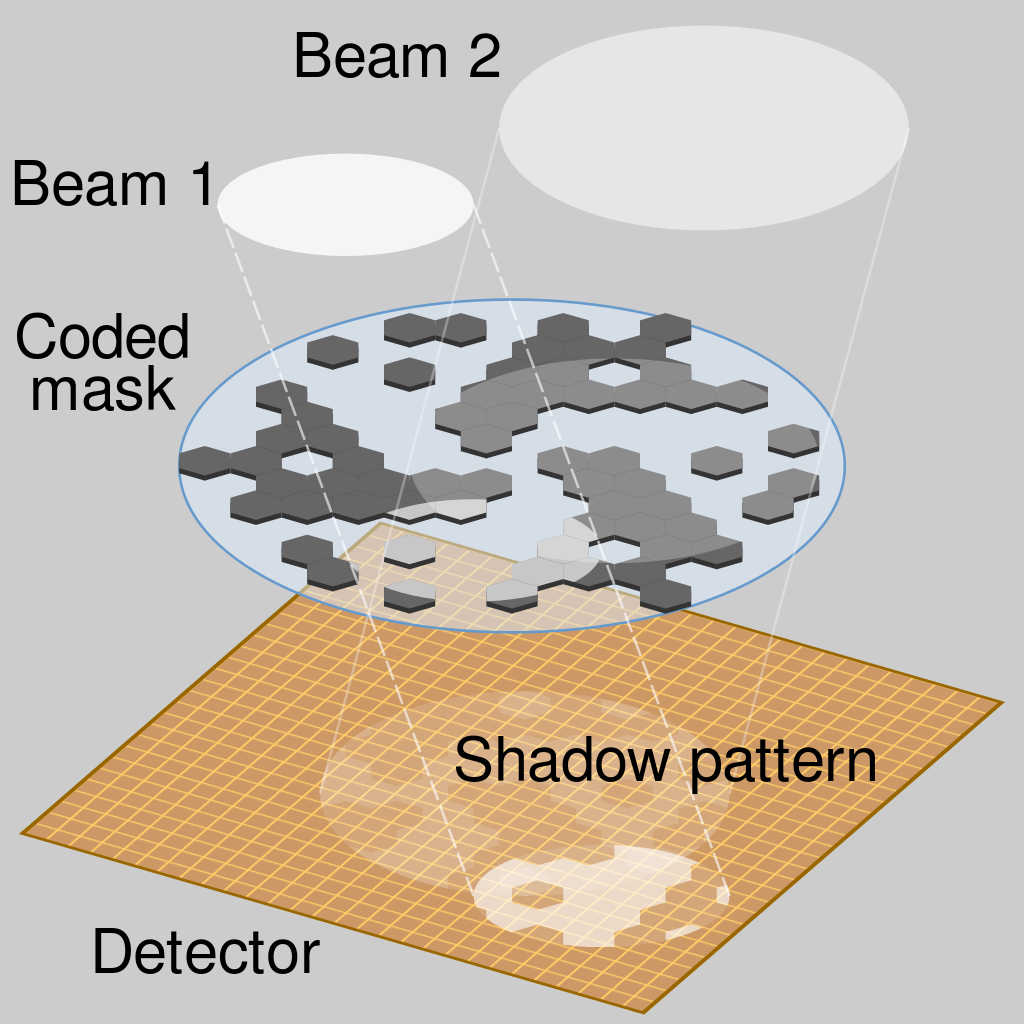
\includegraphics[width=\linewidth]{Images/General/HURA_hexagonal_coded_aperture_mask_principle.svg.png}
  \vspace{-20pt}
  \caption{The effect of SPIs mask on incoming source beams \cite{HURA}.}
  \vspace{-20pt}
  \label{HURA}
\end{wrapfigure}

To further prevent unnecessary background counts in the detectors an anticoincidence shield (ACS) is installed around various of SPIs components (see figure \ref{SPI cut view}). It consists of 91 BGO crystals with a volume of approximately $790\text{cm}^3$ each. Whenever an event is measured simultaneously in the ACS and in the Ge detectors it is vetoed. 



\subsubsection*{Mask}



\begin{figure}
  \centering
  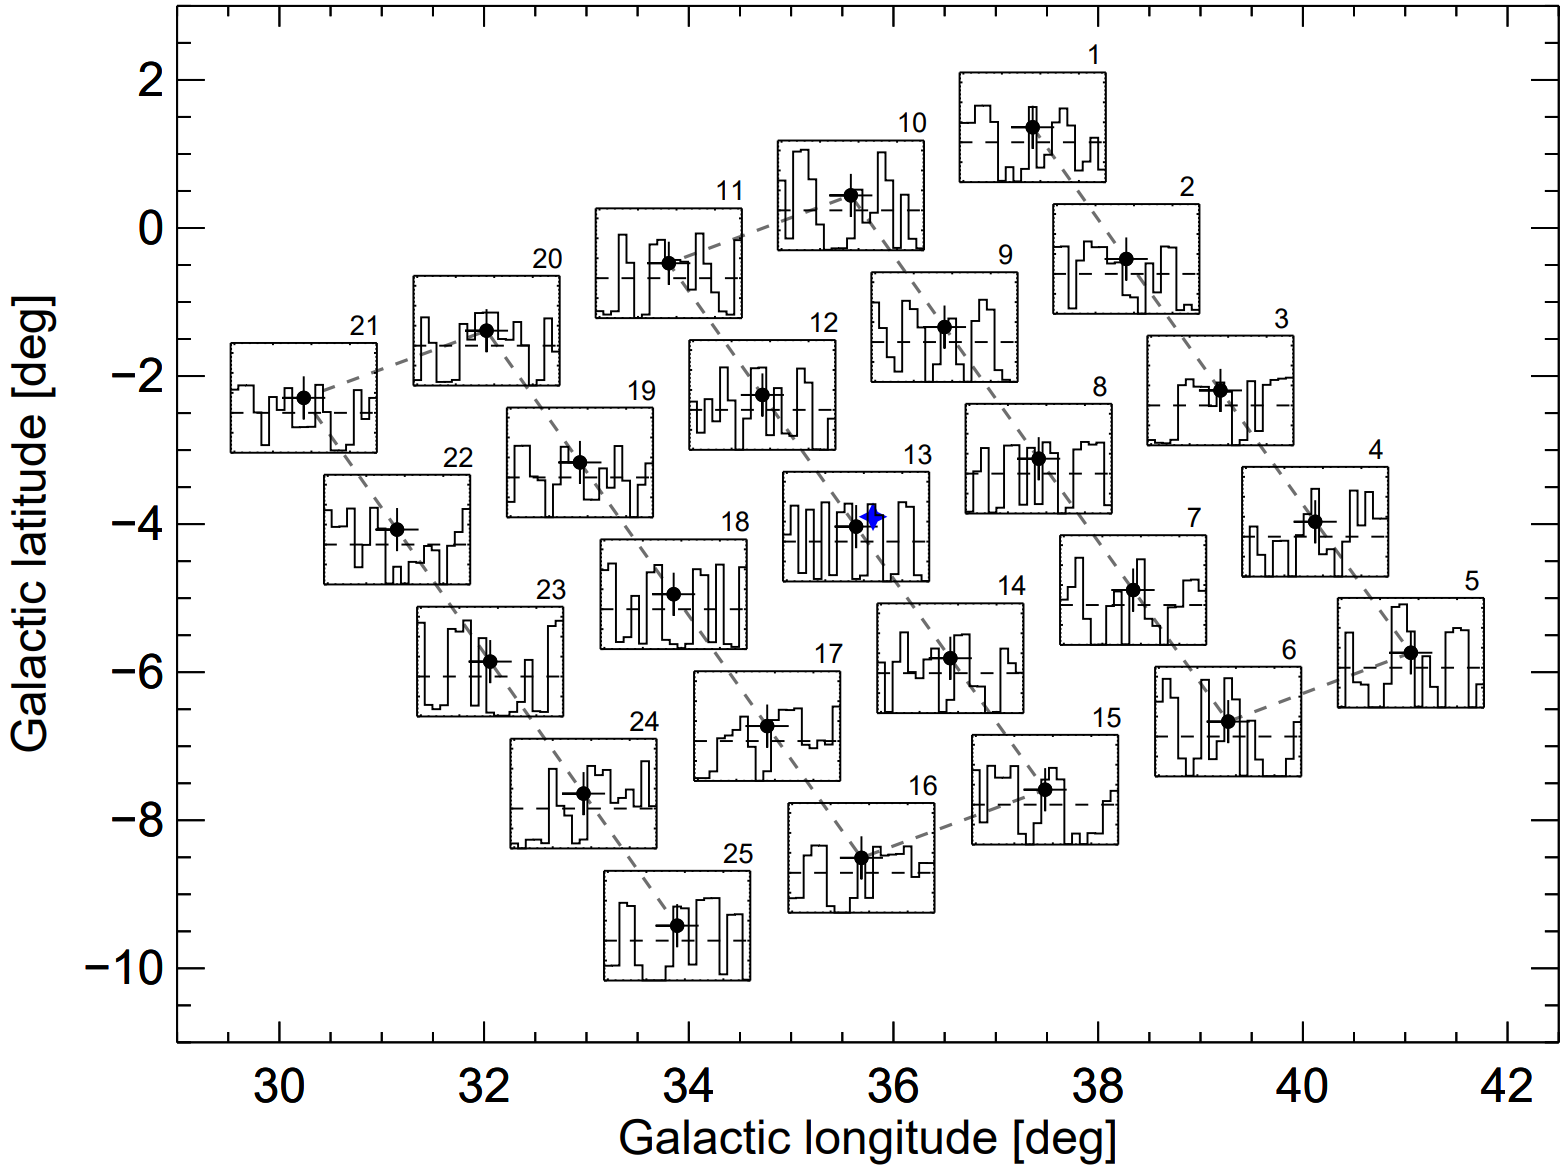
\includegraphics[width=\textwidth]{Images/General/Siegert_PHD_Pointings_pattern.PNG}
  \caption{A typical SPI $5\times5$ grid pointing pattern, each $2.1^\circ$ apart, marked with black dots and sequence number. The blue star in the center represents a celestial source, and the inset panels show the relative detector patterns from the celestial source. A close-up of pointing 13 is shown in figure \ref{spegert_pointings_pattern_close_up}. \cite{dissertation}}
  \label{spegert_pointings_pattern}
\end{figure}

\begin{figure}
  \centering
  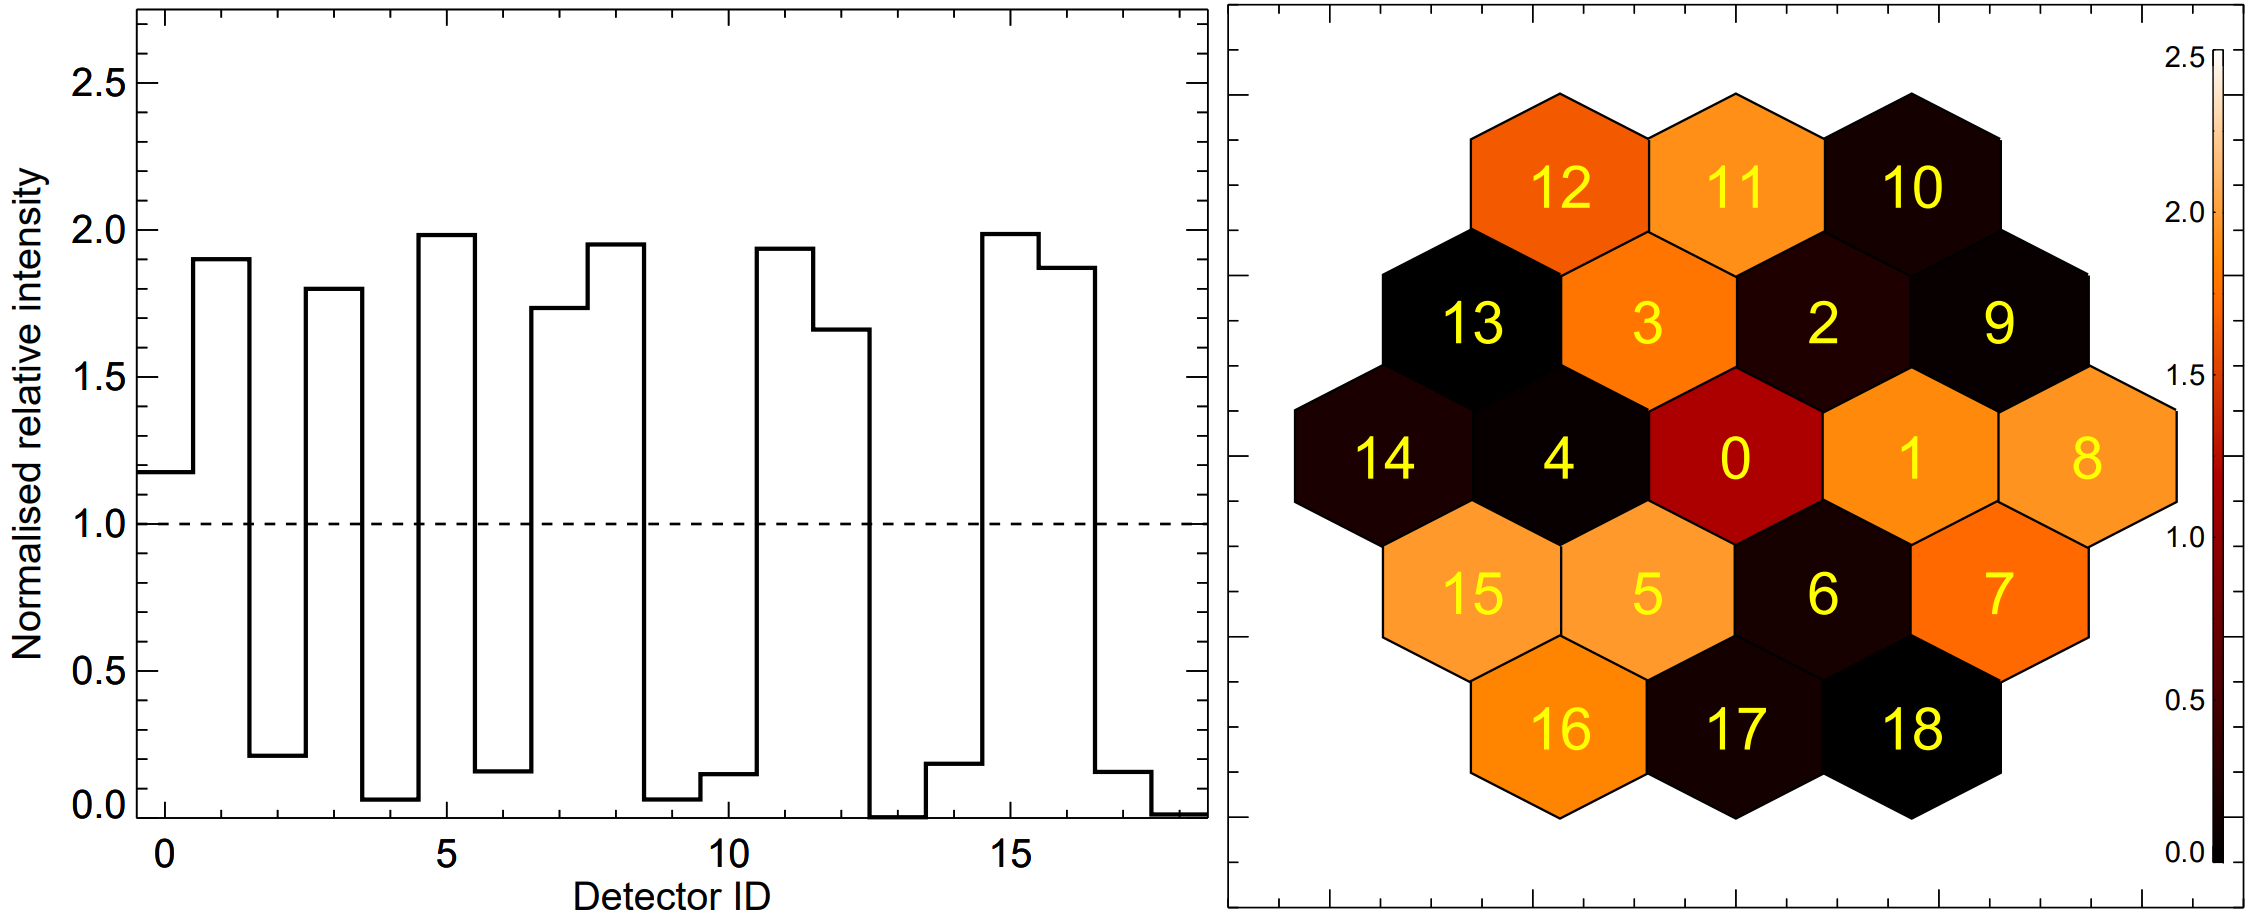
\includegraphics[width=\textwidth]{Images/General/Siegert_PHD_P13.PNG}
  \caption{A close-up of pointing 13 from figure \ref{spegert_pointings_pattern}. On the left we see the relative detector pattern caused by the source in a step plot, and on the right we see the same information displayed as a shadowgram on the detector array. \cite{dissertation}}
  \label{spegert_pointings_pattern_close_up}
\end{figure}

Before any photons can reach the array of detectors, they must pass through the coded aperture mask made of a 3cm thick tungsten alloy, located 1.71m above. The $120^\circ$ rotationally symmetric mask is composed of 127 hexagonal tiles (63 opaque and 64 transparent to gamma radiation in the operating energy range) measuring 60mm side to side, and is inscribed within a circle with 720mm diameter. The effect that the mask has on incoming source beams is illustrated in figure \ref{HURA}, and the way this might influence the number of source counts measured in the detector array is visualized for an example source in figures \ref{spegert_pointings_pattern} and \ref{spegert_pointings_pattern_close_up}. This illustrates how we may infer both the source spectrum and position from the detector counts using multiple offset pointings of an astronomical source.




\subsubsection*{Event Types}
\begin{wrapfigure}{R}{0.55\textwidth}
  \vspace{-20pt}
  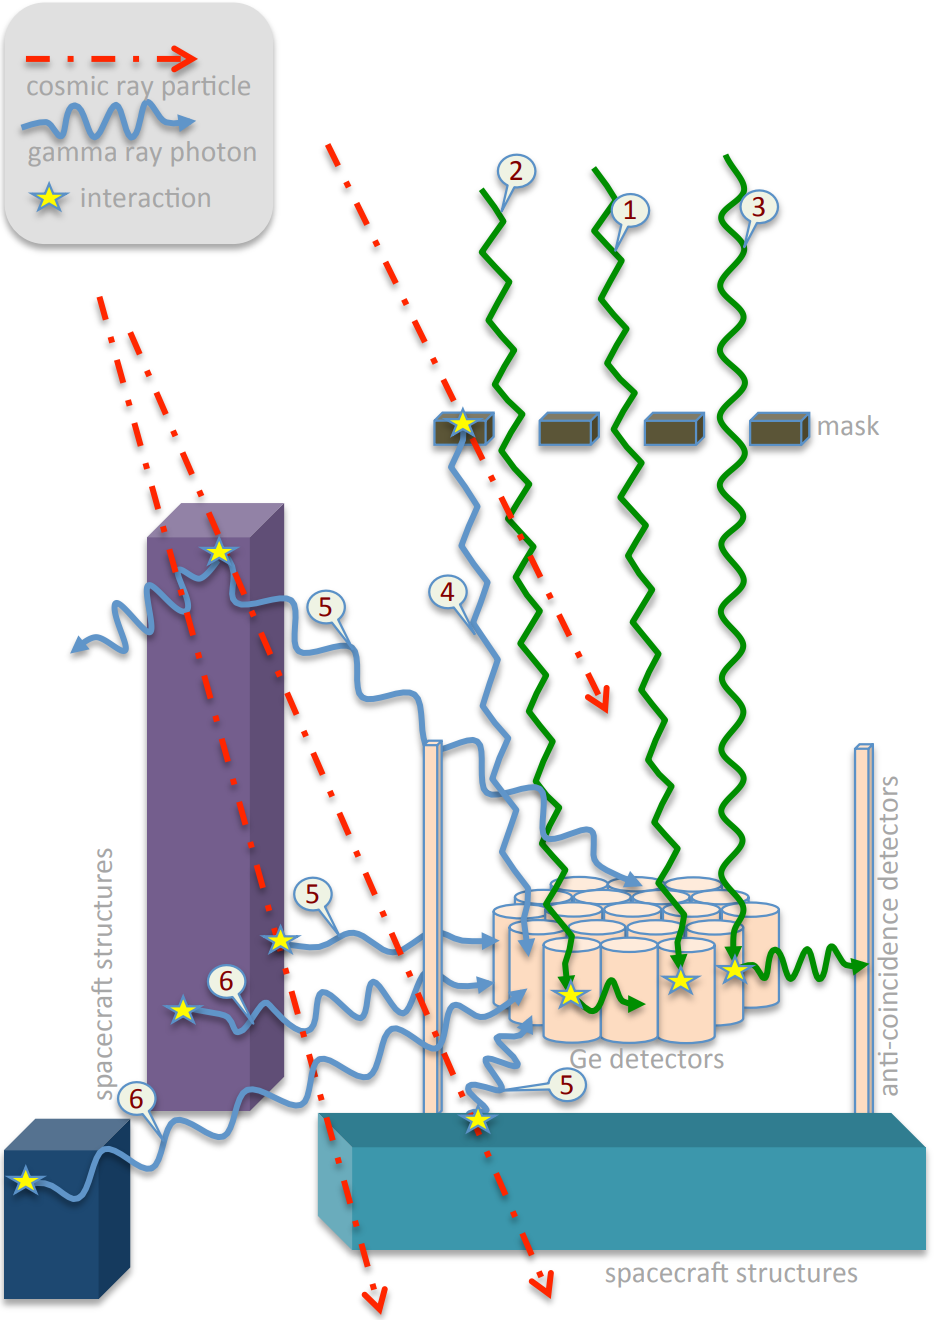
\includegraphics[width=\linewidth]{Images/General/SPI_event_types_roland_2017.PNG}
  \caption{Illustrations of different event types measured by SPI. Incoming source photons (green) may be absorbed in one detector (1), multiple detectors (2), or be self-vetoed by interacting with the ACS (3). Cosmic particles may interact with surrounding structures, resulting in background photons (blue)(4,5,6). Although the ACS helps suppress these events, they still occur. \cite{refId2}}
  \vspace{-50pt}
  \label{event_types}
\end{wrapfigure}

Figure \ref{event_types} shows some of the different event types measured by SPI. These are generally classified in the following categories:

\begin{itemize}
  \item Single Events (SE) - only one of the Ge detectors measured an energy deposit in the relevant time frame. Ideally this photon is fully absorbed in the detector, although there is no way of confirming this.
  \item Multiple Events (ME) - multiple Ge Detectors measured an energy deposit simultaneously. Ideally this is caused by a photon compton scattering to another detector (or multiple detectors), where it is fully absorbed. Again, there is no way of confirming this the photon is fully absorbed or that the measured energies were not coincident from multiple sources.
  \item Pulse Shape Discriminated Events (PE) - A SE for which the PSD electronics also triggered. Since each detector is equipped with its own PSD electronics chain, only SEs can be pulse shape discriminated. Another effect of this implementation is that the SE spectrum will have a reduced count rates in the PSD energy range, where SEs are PSD flagged and thus "removed" from the SE spectrum. 
\end{itemize}

Although the ACS does help with suppressing background and non-fully absorbed photons, it cannot guarantee  anything. In fact, a very large portion of SPIs measured counts are background counts. 

\subsubsection*{Spurious Events} \label{sec spurious events}
SPI also suffers from so called spurious events. These may occur when high-energy deposits are made in the germanium detectors. The analog electronics can become saturated and, due to reasons better explained elsewhere \cite{Roques}, low energy counts will be displaced toward higher energies. However, it has been found that the PSD electronics chain does not suffer from the same issues. This is why it is recommended to use only PEs in the PSD energy domain, and not SEs. 


\section{About Spimodfit} \label{about smf}



Given the complexities discussed above, and many more not discussed, it is clear that working with SPI data is no trivial task. Although SPIs Instrument Response Function (IRF) are readily available to be used, there is no stand-alone background model. Since the background counts dominate source counts in almost all circumstances, it is no surprise that several independent methods to analyze SPI data have been developed. One such method is Spimodfit, developed primarily by Thomas Siegert at MPE \cite{refId1} \cite{SMF_Cookbook}.

\begin{wrapfigure}{R}{0.55\textwidth}
  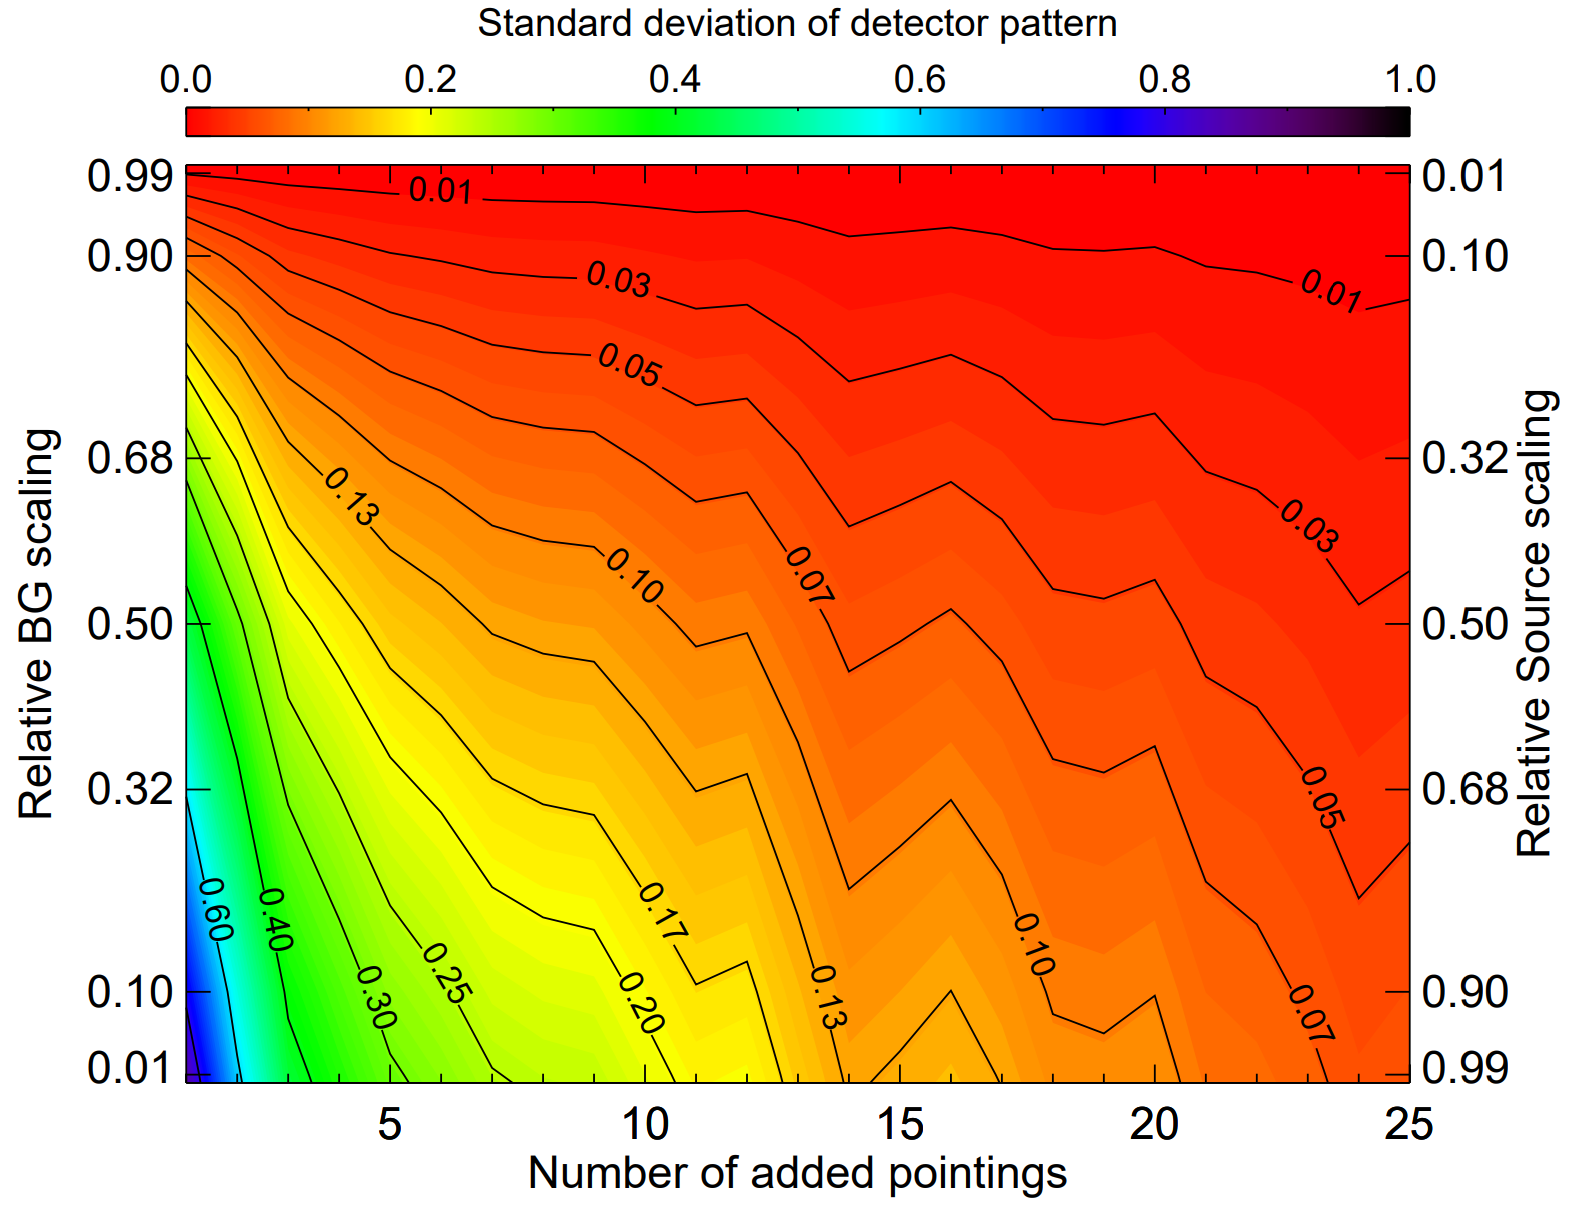
\includegraphics[width=\linewidth]{Images/General/SMF_background_pattern_siegert_2019.PNG}
  \caption{The standard deviation of detector patterns as a function of the number of pointings and the source to background intensity. We see that even very bright sources become almost entirely washed out given enough pointings, and only the sum of the background detector patterns remains. \cite{refId1}}
  \vspace{-0pt}
  \label{smf_background_model_idea}
  \vspace{-5pt}
\end{wrapfigure}

In order to create Spimodfit a detailed background and response database had to be constructed first. The fundamental idea that allows this background database to work is that the detector count-rate patterns of individual isotopes stay constant on all timescales. This means that every process that leads to background counts creates some specific, energy dependent pattern in the detector array which stays constant. These processes are split into parameters for continuum processes as well as many $\gamma$-ray lines. The intensities of these different patterns created by the processes may vary, which is why they are fitted to the relevant count-spectra per energy bin in order to create the background spectrum used in every analysis. This requires one to have knowledge of what the different patterns are. Hence, a database of the detector patterns was created by adding many SPI pointings together over relevant timescales, so that any sources in the pointings are washed out and only the detector patterns remain (see figure \ref{smf_background_model_idea}). Naturally, this very brief description of the Spimodfit background model given here skips over many details and complexities that had to be taken into consideration.

Spimodfit will be used extensively in this thesis as a reference point regarding SPI data fitting.



\section{PySPI and the Goal of this Thesis}
PySPI is a python analysis framework for Gamma-Ray Burst (GRB) data from SPI \cite{Biltzinger2022}. It is designed to take user inputs like the time of the GRB and energy bins, automatically download relevant data files, and to construct a response and time series, which can then be used as a plugin for 3ML \cite{3ml}.

Momentarily, PySPI is only built to work with transient sources. The goal of this thesis is to extend PySPIs functionality to be able to analyze persistent sources as well. Unlike transient sources, whose time-sensitive nature circumvents the need for an accurate background description, persistent sources are not so easily distinguished from background counts and thus do necessitate a way to deal with SPIs dominant background.

\chapter{Theory and Simulation}

\section{General Procedure} \label{General Procedure}
In contrast to previous approaches to working with INTEGRAL SPI, the method of analyzing SPI data developed for this thesis does not attempt to construct a background model, and instead uses a profile likelihood to eliminate its effect in the source model fit. The underlying assumption that allows this to work is that background count rates in each energy bin per detector remain constant for temporally and spatially near SPI Science Windows (SCWs) (also called pointings). Neighboring SCWs are thus grouped into clusters of assumed constant background count-rates, allowing for a source model to be fitted to the data using the likelihood calculations described below. Just like in chapter \ref{Introduction}, we distinguish between source counts, which describe all detected events directly originating from astronomical objects considered in our source model, and background counts, which describe all other detector events.

\subsection{Likelihood Calculation}

Once we have split our set of SCWs into clusters within which we claim the assumption of constant background to be true and have defined a source model, a likelihood value can be calculated for each energy bin of each detector in each cluster. If one energy bin of one detector in one SCW with measuring time $t$ has a source count rate $s$ and a background count rate $b$, the probability $P$ of measuring $C$ counts follows a Poisson distribution:
\begin{equation}
    P(C \vert b, s, t) = \frac{\left( t \left( b + s \right) \right) ^C \text{exp}\left( -t \left( b+s\right)\right)}{C!}
\end{equation}

Equivalent energy bins in the same cluster are assumed to have the same background count rate $b$, so that the probability of measuring $C_1$ counts in one SCW and $C_2$ counts in another SCW is simply:

\begin{equation}
    P(C_1, C_2 \vert b, s_1, t_1, s_2, t_2) = P(C_1 \vert b, s_1, t_1) \cdot P(C_2 \vert b, s_2, t_2)
\end{equation}

The likelihood $\mathcal{L}$ for any energy bin of a detector within a cluster depends on all equivalent energy bins in that cluster, i.e. one term for each SCW in the cluster. If we have cluster of size two, the likelihood is described by:

\begin{equation}\label{log likelihood}
    \text{ln}\mathcal{L}(C_1, C_2, t_1, t_2\vert b, s_1 s_2) = \text{ln}P(C_1 \vert b, s_1, t_1) + \text{ln}P(C_2 \vert b, s_2, t_2)
\end{equation}

This expression allows us to solve for the probability distribution of $b$. A full and mathematically correct treatment of the background parameter $b$ turns out to be very cumbersome with only marginal benefits. Hence, the profile likelihood is used by simply solving for the background count rate value $b_M$ which maximizes the likelihood. This is easily done by setting the derivative of equation \ref{log likelihood} to zero and solving for $b$. For a cluster size of two one finds:
\begin{equation} \label{eq: max lik back}
    b_M = \frac{1}{2} \left[ \frac{C_t}{t_t} - s_t + \sqrt{\left( \frac{C_t}{t_t} - s_t\right)^2 + 4 \left( \frac{C_1s_2+C_2s_1}{t_t}-s_1s_2\right)}\right]
\end{equation}
where $C_t=C_1+C_2$, $s_t=s_1+s_2$, and $t_t=t_1+t_2$. Using this maximum likelihood background $b_M$ finally allows us to compute a likelihood value that is only dependent on the measured counts and the source model:
\begin{equation} \label{log_likelihood final}
    \text{ln}\mathcal{L}(C_1, C_2, b_M, t_1, t_2 \vert s_1, s_2) = \text{ln}P(C_1 \vert b_M, s_1, t_1) + \text{ln}P(C_2 \vert b_M, s_2, t_2)
\end{equation}
The process for clusters with sizes larger than two is analogous. One such likelihood value exists for every energy bin of every detector in every cluster, such that the total likelihood value for any given source model is simply the sum of the logarithmic likelihoods over all energy bins, detectors, and clusters:

\begin{equation} \label{total log likelihood}
  \text{ln}\mathcal{L}_{\text{total}} = \sum_{\text{Clusters}}\sum_{\text{Detectors}}\sum_{\text{Energy-Bins}} \text{ln}\mathcal{L}(C_1, C_2, b_M, t_1, t_2 \vert s_1, s_2)
\end{equation}

Thus the source model may be fitted to the count data by applying an algorithm to maximize the likelihood. In this case Multinest \cite{Feroz_2019} is the bayesian inference algorithm of choice.

An important detail is that the expected value of the maximum likelihood background is equal to the true background rate:
\begin{equation}
  E(b_M) = b
\end{equation}
Depending how the random samples of the poisson distributions are drawn, it is possible for the maximum likelihood background to be less than zero $b_M<0$. One might be tempted to impose a lower limit of 0 since the physical background rate cannot be lower than 0, but this would actually be a big mistake since the introduced asymmetry means that the expected value of the maximum likelihood background is no longer equal to the true rate $E(b_M) \neq b$, which in turn prevents a bayesian fitting algorithm from correctly determining the true source parameters.


\subsection{General Procedure: Summary}

The general procedure for fitting persistent sources with PySPI can thus be summarized in the following steps:
\begin{enumerate}
  \item Select all relevant SCWs to be used in the analysis. Usually this is done on a revolution basis, so that all SCWs from the used INTEGRAL revolutions are included, provided SPIs orientation is sufficiently close to the source in question.
  \item Group the relevant SCWs into clusters. These should preferably have only a small time difference and angular distance in SPIs orientation between them so that the assumption of a constant background rate in every energy bin of every detector is justified. Refer to appendix \ref{Clustering Algorithm} for more details on the clustering algorithm developed for this purpose. In principle, clusters of any size ($>1$) can be used, although only cluster-sizes 2 and 3 have been implemented and tested. Clusters of size 2 are most commonly used since they are generally the easiest to work with due to the constant background assumption and computational speeds.
  \item Set-up a source model to be fitted to the data using the python package astromodels \cite{astromodels}. The built in SPI response function capabilities of PySPI allow one to easily calculate the count rates based on the model.
  \item Set-up equation \ref{total log likelihood} so that the multinest bayesian fitting algorithm can vary the source model parameters to maximize the total likelihood. Then run the fit.
  \item If deemed necessary conduct a posterior predictive check (PPC) analysis (see chapter \ref{sec:PPC Back}) to verify the the fit quality and check if the assumption of constant background rates is well met. It is a common occurrence for some clusters to not have constant (or constant enough) background rates. These are easily identified in the PPC CDFs, so that they may be removed from the list of clusters for the fit to be run again.
\end{enumerate}



\section{Pure Simulation}\label{sec: pure sim}
Before any real sources are fitted, it makes sense to test the SPI fitting method on a purely simulated count spectrum. This not only allows us to see exactly how well the fit performs since we know the true model parameters of any sources in the simulated spectrum, but it also allows us to test under which conditions the fit may or may not fail.

To begin a simulated count spectrum is required, consisting of source and background counts. For the following simulations this is done in the following way, unless otherwise specified:

\begin{enumerate} 
  \item Choose a real SPI revolution as a baseline. It is mostly irrelevant which revolution is chosen. For this analysis revolution 0374 is used. We will use the SPI orientations of the SCWs in this revolution as the orientations of our simulated SCWs in order to achieve realistic conditions. 
  \item \label{step pure sim back}Generate a background spectrum. In order to have a realistic background spectrum, the background counts from one SCW are taken and duplicated to all other SCWs and then poisson distributed. The lifetimes (total active measuring time of each detector in each SCW) for each SCW are also duplicated to match each other. This way the background count rates are identical for all SCWs, yet also realistic, in the sense that the spectrum could that of an actual SPI SCW.
  \item Define spectrum of the source to be simulated, as well as position. In this case powerlaws as shown in equation \ref{powerlaw} are used, and the position of the sources is chosen to be central to as many SCWs in the revolution as possible ($RA=10^\circ, DEC=-40^\circ$ in equatorial coordinates). Although the exact parameters used in the following sections will vary, most powerlaw spectra are chosen to be comparable to the Crab Nebula in terms of luminosity and index.
  \item Use the SPI Instrument Response Function (IRF) to calculate the expected source count rates in each energy bin in each detector for each SCW. Multiply these by the respective lifetimes (effectively the active measuring time) of the detectors in the SCWs, and finally draw a sample of a Poisson distribution with the respective means to attain the measured counts of the simulated source for each energy bin in each detector in each SCW.
  \item Add the source counts to the background counts to acquire the total counts.
\end{enumerate}

To measure the quality of a fit we shall use the Mahalanobis distance:

\begin{equation}
  d_M = \sqrt{(\vec{V}_F - \vec{V}_T)^TS^{-1}(\vec{V}_F-\vec{V}_T)}
\end{equation}

which tells us the number of standard deviations the fitted source values $\vec{V}_F$ are away from the true source values $\vec{V}_T$, where $S$ is the covariance matrix.

Unless otherwise specified, the following fits utilize an energy range of 18-2000keV. Since this is purely simulated data we do not need to worry about spurious events or any other anomalies in the SPI data-space. In order to visualize the results we may plot the confidence intervals of the posterior parameter distributions next to the true source parameters, which we know exactly due to having simulated the sources. Unless otherwise specified, the confidence intervals of one standard deviation are used.

\subsection{Consistency, Accuracy, and Precision}

\begin{figure}[h]
  \centering
  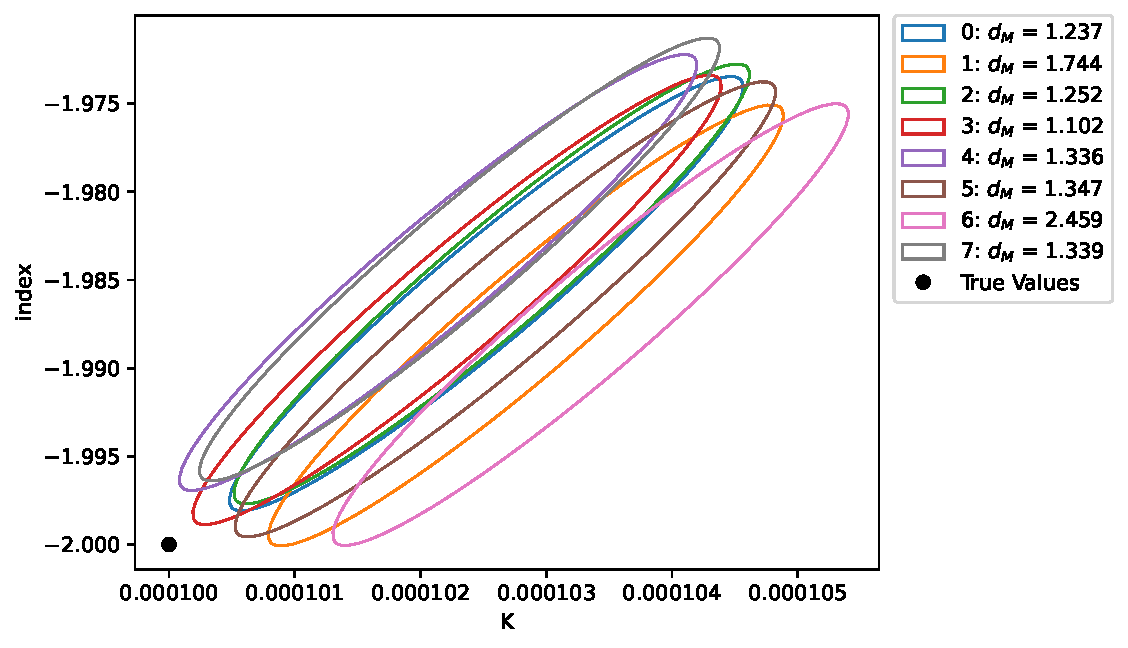
\includegraphics[width=\textwidth]{Images/Pure_Simulation/combined_plot_repeated_identical.pdf}
  \caption{Repeated fits for exactly identical datasets.}
  \label{fig ident}
\end{figure}

The first test is how consistent the fitting is with exactly identical inputs. The results are shown in figure \ref{fig ident}, where the same source is fitted 8 times. We see that the results are all very similar. However, since the inputs are exactly identical, it is surprising that the multinest fitting algorithm still has deviations this significant, ranging from 1.1 to 2.4 standard deviations away from the true values. 

\begin{figure}[h]
  \centering
  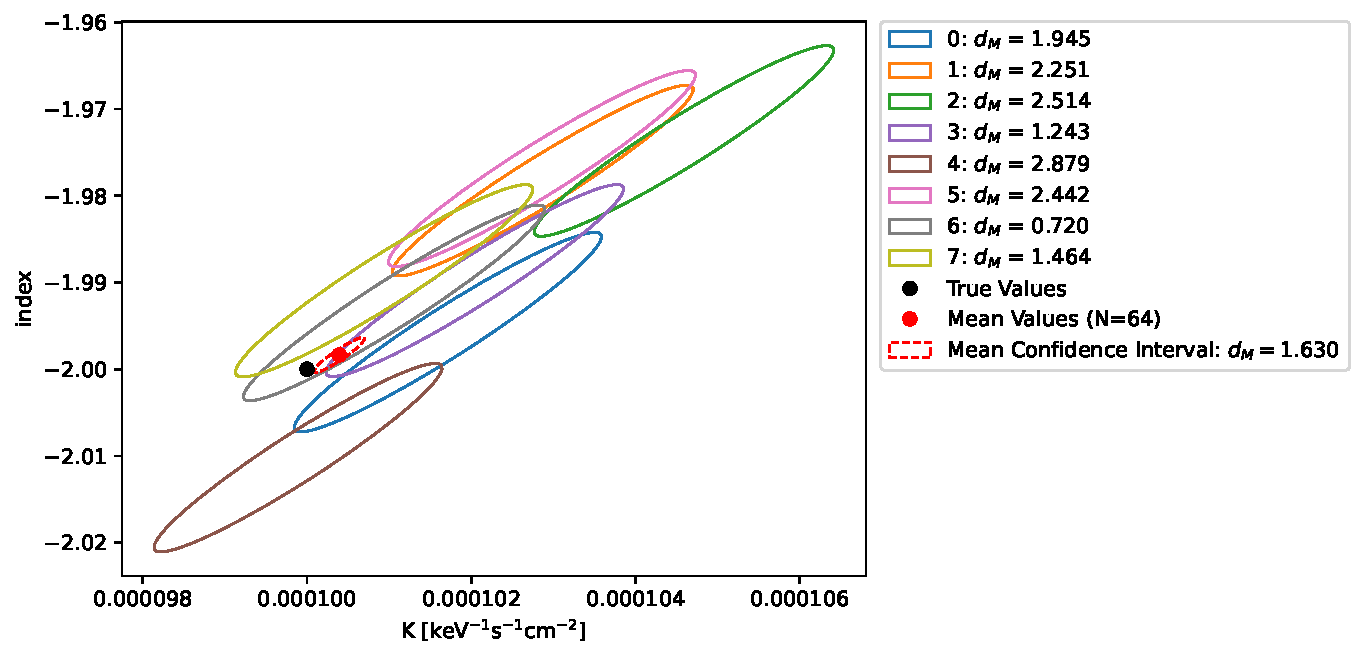
\includegraphics[width=\textwidth]{Images/Pure_Simulation/combined_plot_repeated_identical_new_gen.pdf}
  \caption{Repeated fits for newly generated datasets, using the same exact same baseline before random poisson samples are drawn in the dataset generation. Also shown is the mean fit value for 64 fits (only 8 shown here), as well as the confidence interval of said mean.}
  \label{fig ident new gen}
\end{figure}

Although the previous test gave us great insight into the consistency of the fits, it told us nothing about their accuracy. To test this we have to regenerate the simulated source spectrum, so that every random poisson sample is redrawn. The results of this are shown in figure \ref{fig ident new gen}. As expected, the results are now distribution with much greater variance around the true values. Based on the 8 fits shown, the suspicion of a systematic error may arise. This is why this process (generating a new count spectrum and fitting it) was repeated a total of 64 times. We see that the mean values of these 64 fits, and the confidence interval of the mean (taking the sample variance and the variance of individual fits into consideration) match the true values well at 1.63 standard deviations distance. We may thus conclude that we do not have a statistically significant systematic error, at least for the parameters used to set-up this fit.


\begin{figure}[h]
  \centering
  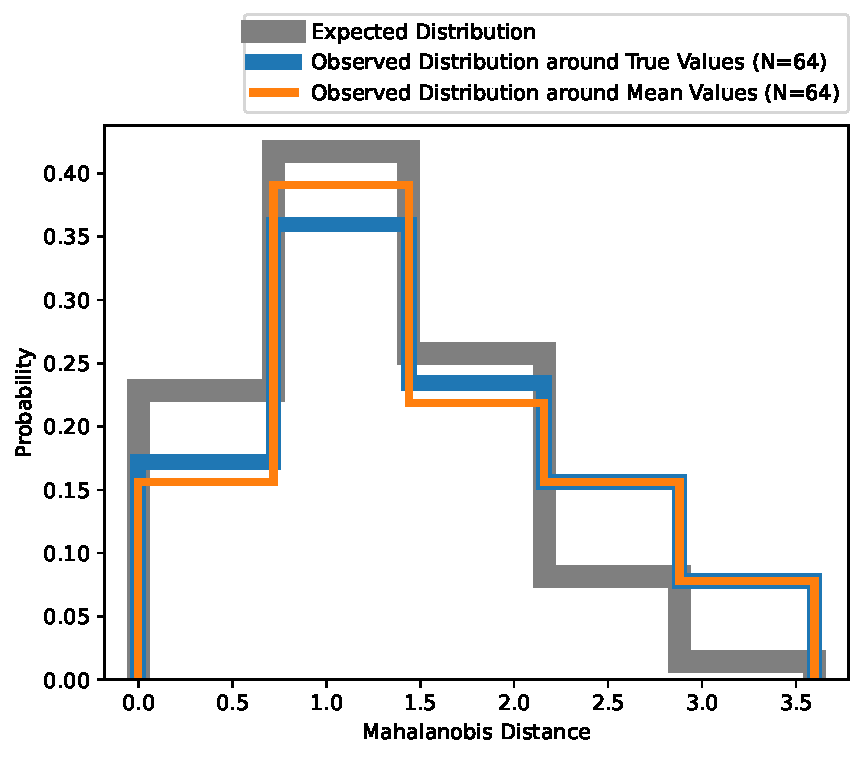
\includegraphics[width=0.65\textwidth]{Images/Pure_Simulation/d_M_distribution.pdf}
  \caption{The distribution of Mahalanobis distances from the 64 fits from figure \ref{fig ident new gen} compared to the expected distribution from equation \ref{d_M exp}. Also shown is the distribution of Mahalanobis distances around the mean values from the 64 fits, instead of the true values.}
  \label{fig d_M distribution}
\end{figure}


Finally we want to test the precision of the fits, i.e. how well the uncertainties of the posterior parameters distributions match their distribution around the true values. Approximating the posterior distributions as gaussian (a fair assumption in this case), the probability of a two-dimensional fit to be between $x_1$ and $x_2$ standard deviations away from the true values is:
\begin{equation} \label{d_M exp}
  P(x_1<d_M<x_2) = \frac{\int_{x_1}^{x_2}x \text{exp}(-\frac{1}{2}x^2)}{\int_{0}^{\inf}x \text{exp}(-\frac{1}{2}x^2)} = \text{exp}(-\frac{1}{2}x_1^2) - \text{exp}(-\frac{1}{2}x_2^2)
\end{equation}
We may thus compare the distributions of the Mahalanobis distances from our 64 fits (figure \ref{fig ident new gen}) to the expected distributions, as is done in figure \ref{fig d_M distribution}. Although the distributions match fairly well, we do see a significant shift towards higher Mahalanobis distances than expected. It appears that our fitting procedure has has a slight tendency to underestimate its posterior uncertainties. That being said, a sample size of 64 is not large enough to definitively support this claim.

Figure \ref{fig d_M distribution} also shows the distributions of Mahalanobis distances around the mean values of the 64 fits, as opposed to the known true values. After Bessel correcting the fit variances to adjust for biases in the sample mean we see a nearly identical distribution, further supporting the claim that there is no systematic error in the fit. 


\subsection{Energy Range}

\begin{figure}[h]
  \centering
  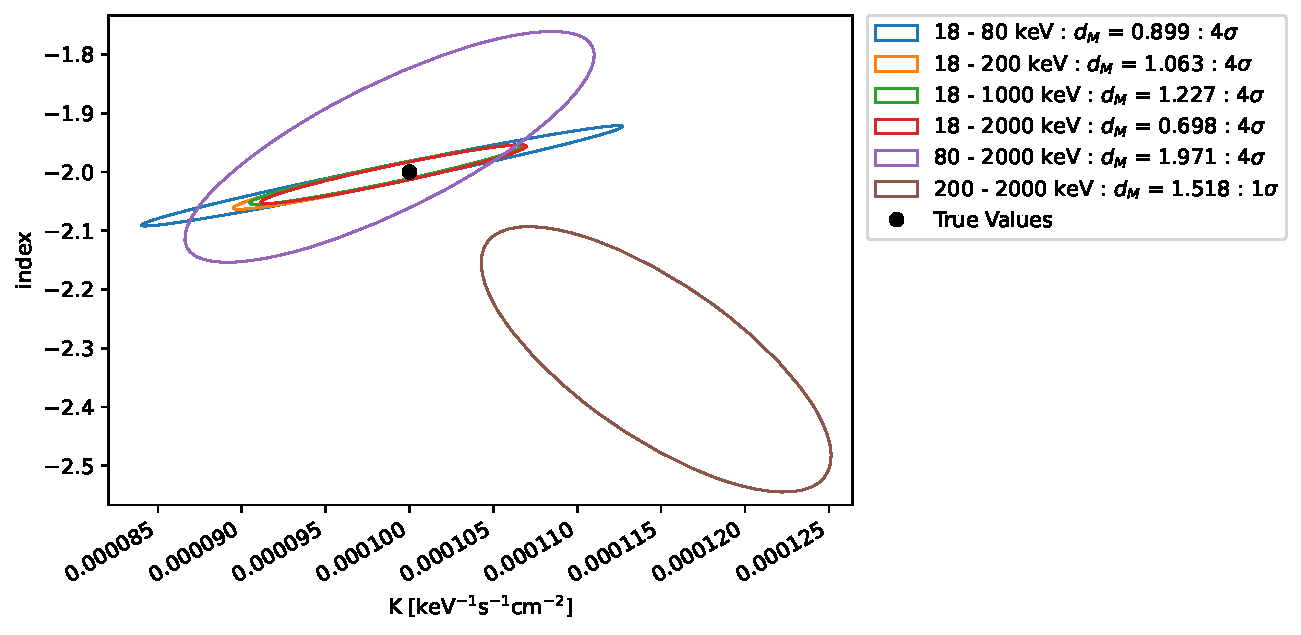
\includegraphics[width=\textwidth]{Images/Pure_Simulation/combined_plot_energy_range.pdf}
  \caption{Identical dataset fitted using only the specified energy ranges. Also note the different number of standard deviations shown in the confidence intervals.}
  \label{fig energy range}
\end{figure}

Figure \ref{fig energy range} shows an identical dataset fitted using different energy ranges. The results are very similar except for fits only going up to 80keV or starting from 80keV or above. Considering a Crab-like source will have its most relevant source counts below 200keV (see figure \ref{fig back spec}) this is not very surprising. It is also worth noting that despite the uncertainties of the fits showing large differences, the number of standard deviations from the true values remains comparable. 




\subsection{Number of Energy Bins}

\begin{figure}[h]
  \centering
  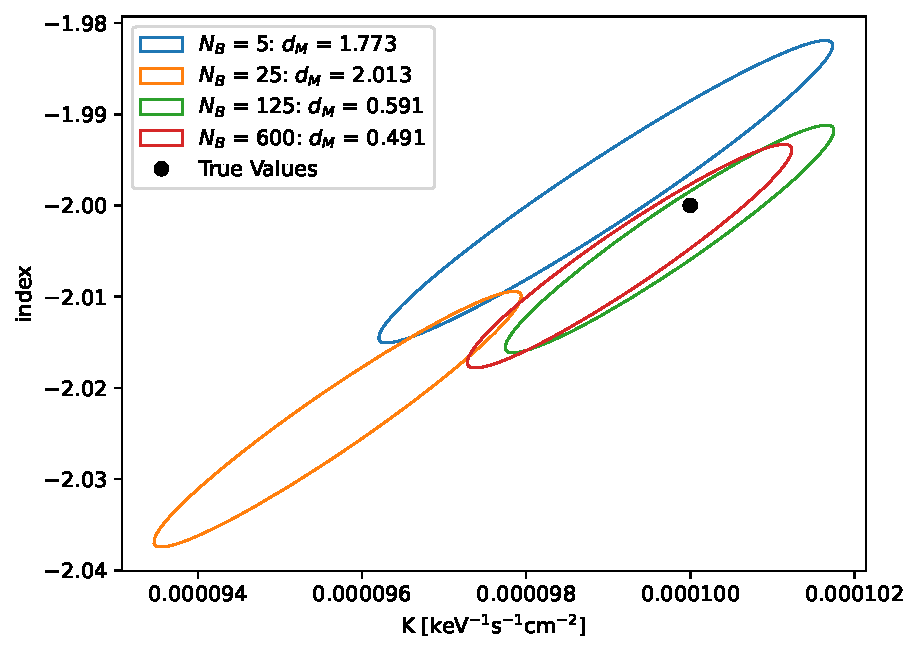
\includegraphics[width=0.65\textwidth]{Images/Pure_Simulation/combined_plot_num_e_bins.pdf}
  \caption{Identical dataset fitted using different numbers of energy bins $N_B$.}
  \label{fig num bins}
\end{figure}

Due to the decreasing number of counts from both source and background at higher energies, the spectra are re-binned into logarithmically spaced bins. Figure \ref{fig num bins} shows what happens when we vary the number of logarithmically spaced bins used. As one might expect, we see no significant differences, except that the uncertainty for 5 energy bins is very slightly larger than for the other fits.


\subsection{Fitting Different Powerlaws}

\begin{figure}[h]
  \centering
  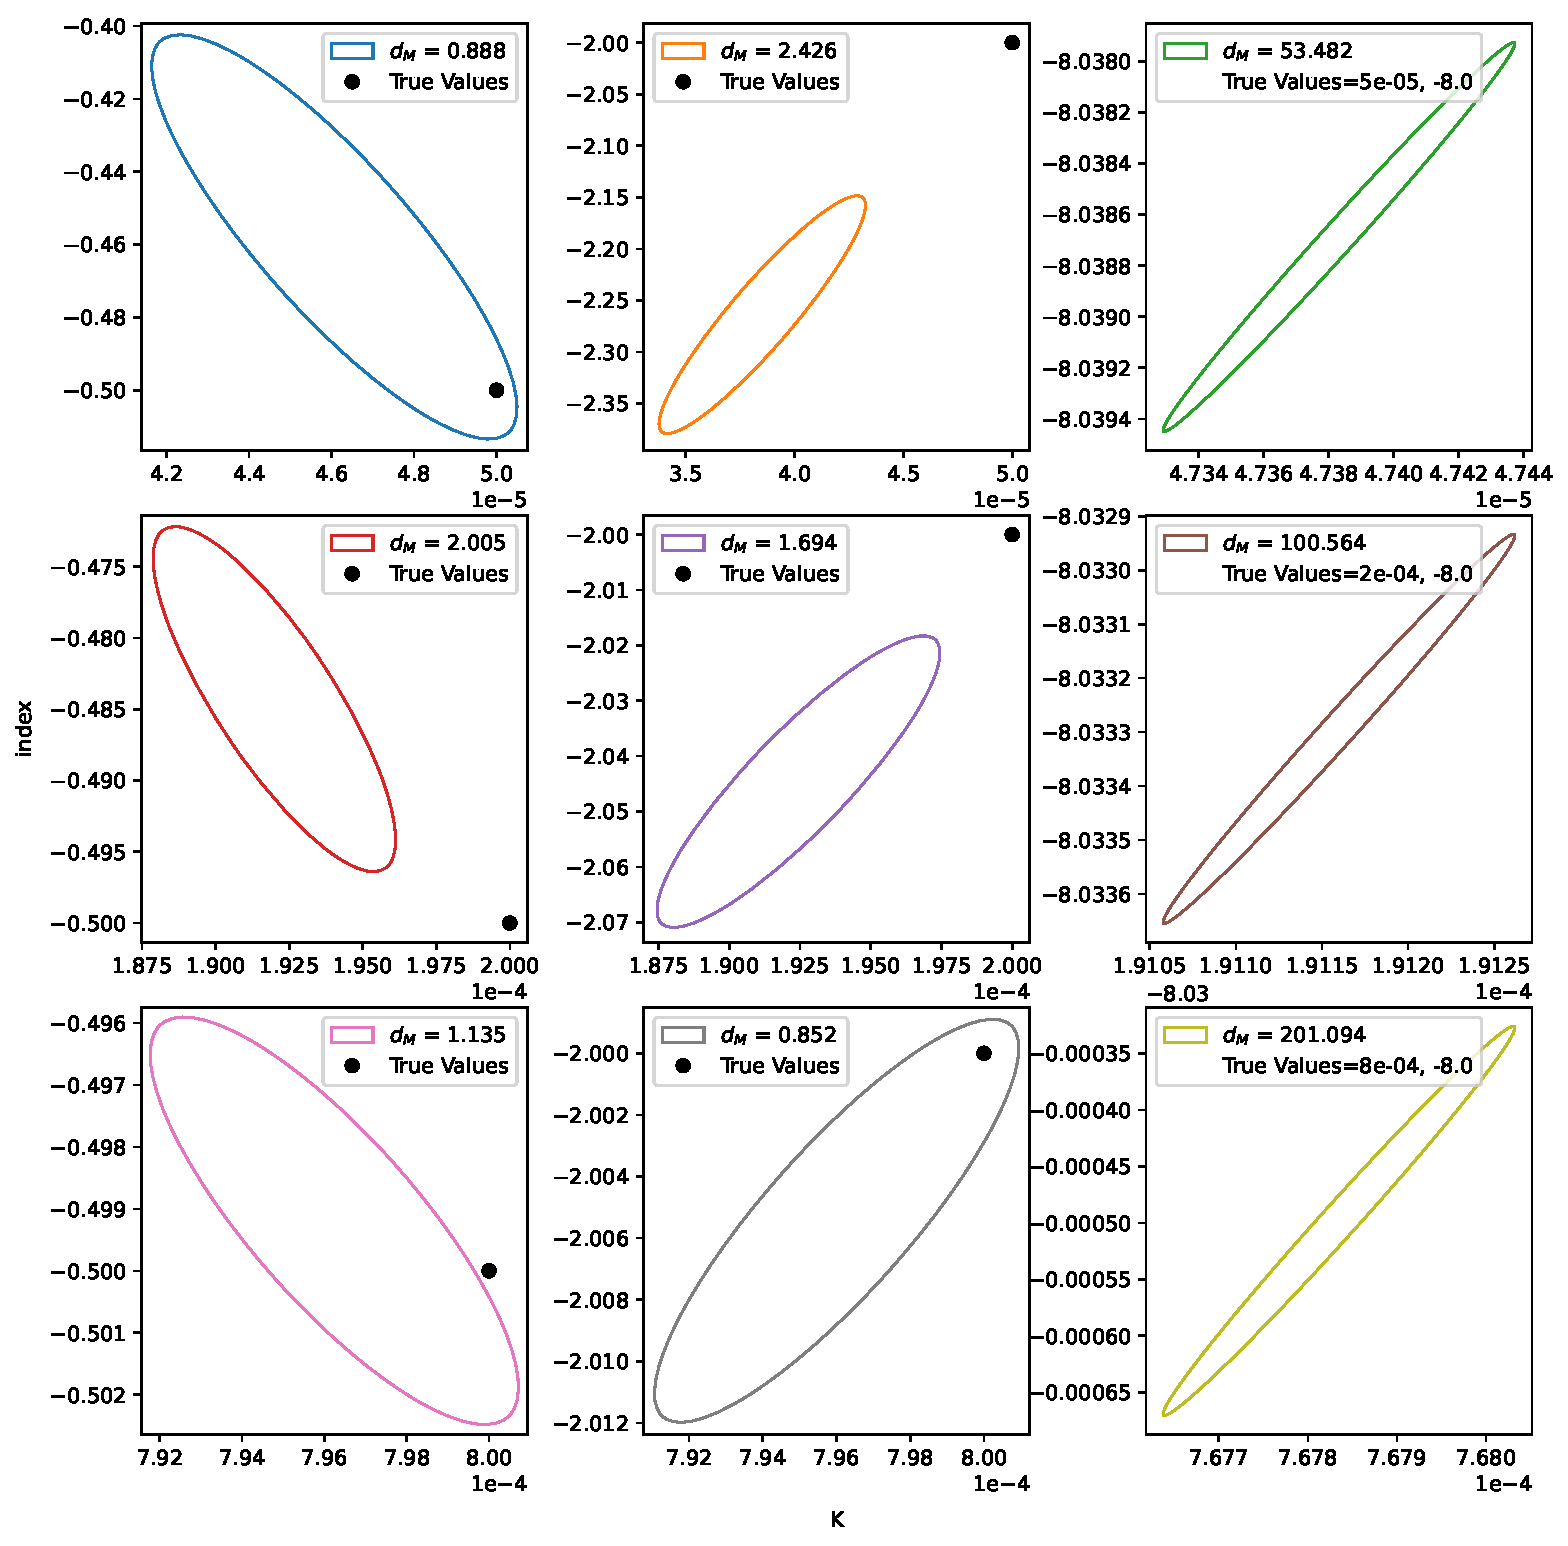
\includegraphics[width=\textwidth]{Images/Pure_Simulation/combined_plots_different_sources.pdf}
  \caption{Count spectra with different simulated powerlaw sources fitted. The source luminosity is changed across the different rows and the source index is changed across columns. The pivot value of the powerlaws used is at $piv=100$keV, meaning that the central plot of the bottom row shows a Crab-like source.}
  \label{fig diff powerlaws}
\end{figure}

So far only Crab-like powerlaws have been fitted. What happens when we change the powerlaw index or reduce the luminosity of the source? According to figure \ref{fig diff powerlaws}, the posterior uncertainties increase for dimmer sources but the accuracy is unchanged as expected. 

The exception to this are steep powerlaws with $index=-8$, for which the fit presents large systematic errors. This behavior is caused by the SPI response matrix. Increasing the number of energy bins for both the model energy bins and the number of SPI-data energy bins causes the error to disappear, as shown in figure \ref{fig large index}. The original SPI response functions are measured at 51 different energies across SPIs wide energy range from 20keV to 8MeV. PySPI then interpolates these original response functions to suitably match both model and data energy bins of choice. For the time being it is unclear whether the systematic error at large indices is a result of an error in the interpolation algorithm of the PySPI response functions, or simply a result of having to do the interpolation in the first place. Regardless, the error does not occur at source spectra with smaller indices, like the Crab Nebula with $index\approx-2$. Furthermore, the error can easily be avoided by using larger response matrices whenever large indices need to be fitted.


\begin{figure}[h]
  \centering
  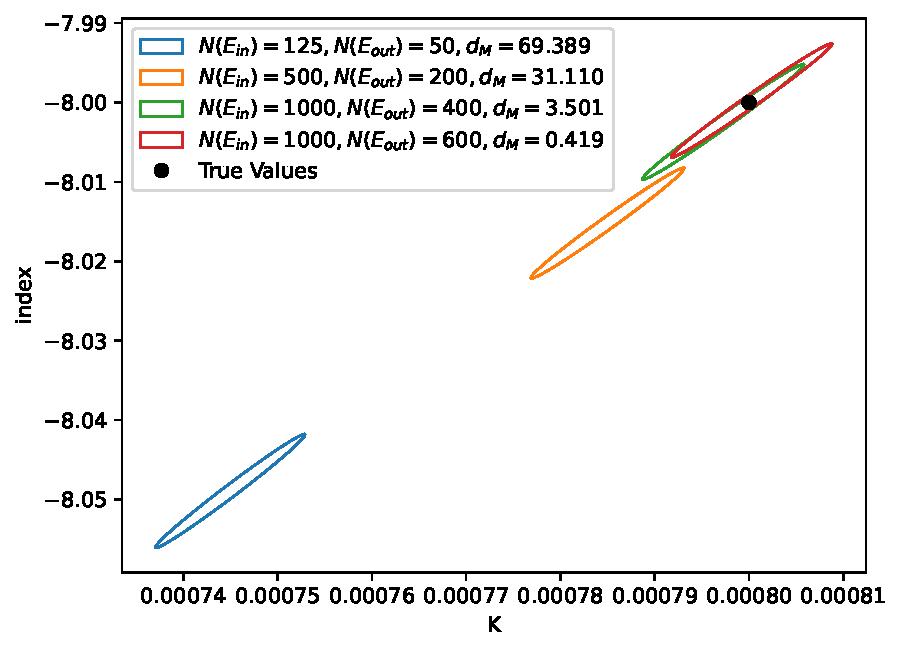
\includegraphics[width=0.6\textwidth]{Images/Pure_Simulation/large_index_combined_plot_10sig.pdf}
  \caption{Powerlaw with $index=-8$ fitted using response matrices of different sizes. $N(E_{in})$ describes the number of energy bins used to describe the source model and $N(E_{out})$ the number of energy bins used for the SPI counts. The confidence interval ellipses show 10 standard deviations each.}
  \label{fig large index}
\end{figure}


\subsection{Second Source}

\begin{figure}[h]
  \centering
  \makebox[\textwidth][c]{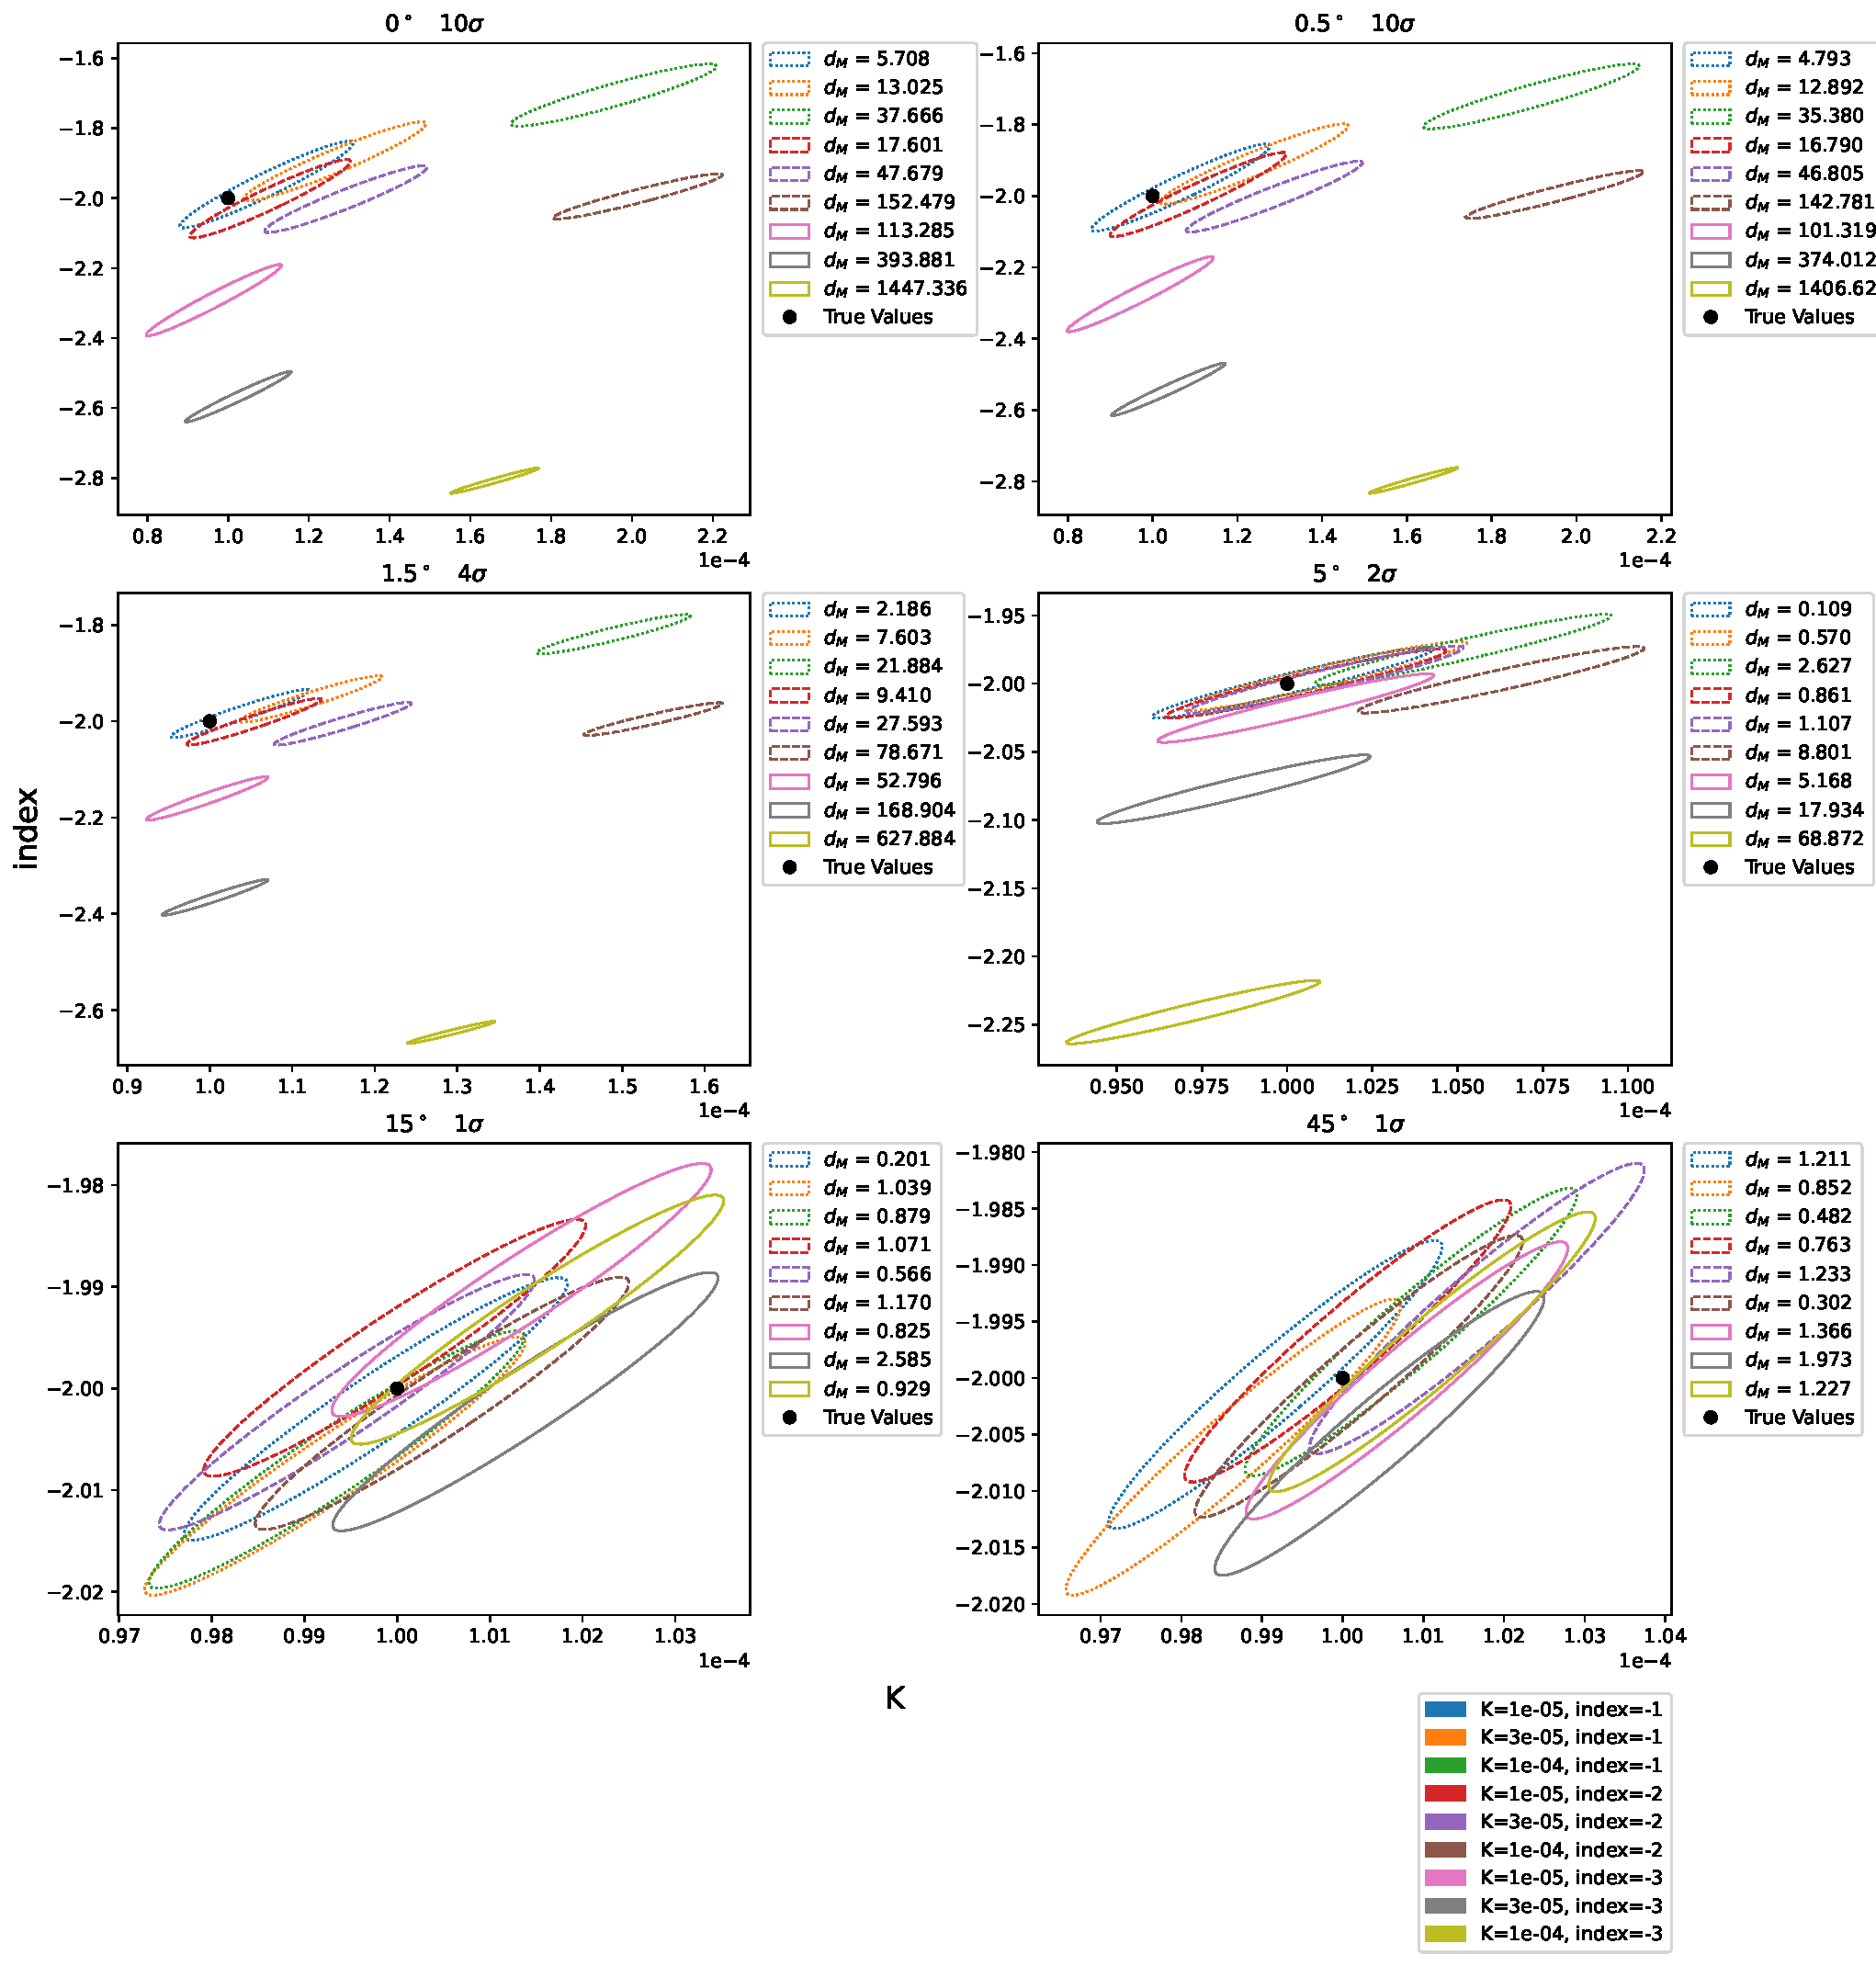
\includegraphics[width=1.1\textwidth]{Images/Pure_Simulation/combined_plots_second_source.pdf}}%
  \caption{The effects of a second source, which is not included in the source model of the fit, on the quality of the fit for the primary source. The different plots show results for different angular distances between the two sources, as stated in the respective titles. The titles further show the amount of standard deviations illustrated by the ellipses. Finally, see the legend at the bottom right for the powerlaw parameters of the second source. All powerlaws are normalized at $piv=200$keV.}
  \label{fig sec source}
\end{figure}

In practical applications there are almost always going to be additional sources within SPI's field of view that are not considered in the source model. This invalidates the assumption that background count rates are constant in corresponding bins within clusters. In order to judge the severity of this, we shall simulate a second source within SPI's field of view (not included in the source model) to observe to ramifications of the fit on the primary source, as is shown in figure \ref{fig sec source}. 

When the two sources are close to each other, the normalization and index shift in accordance to the second source as expected. At 5 degrees apart most fits start to achieve a decent level of quality, and at 15 degrees or more the impact is negligible. The impact is largest when the second source has a large (on an absolute scale) index. We conclude that it is very important to included all sources within $5^\circ$ and luminosity larger than 10\% of the primary source.


\subsection{Data Scaling}

\begin{figure}[h]
  \centering
  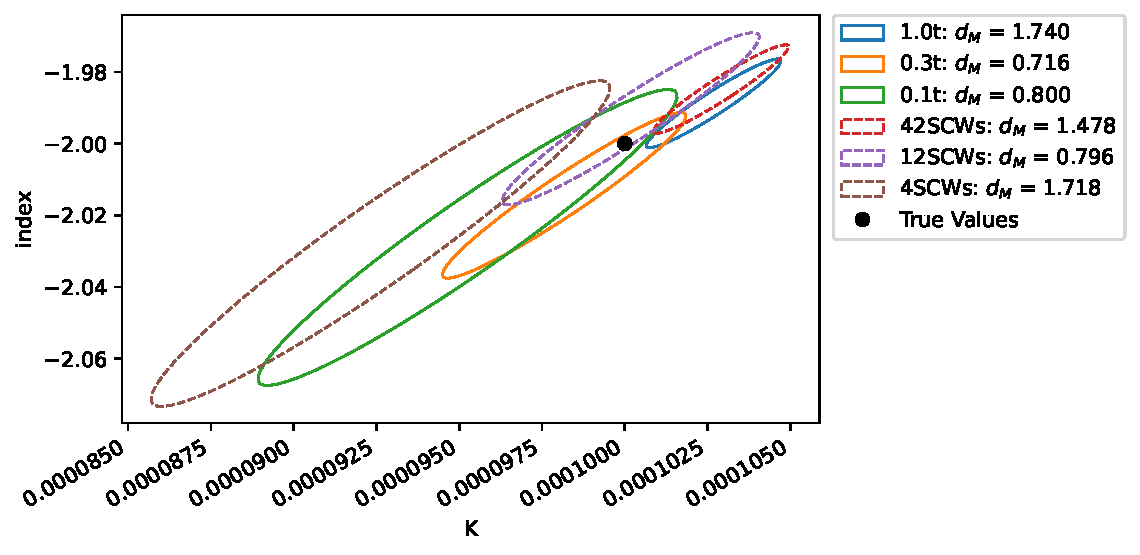
\includegraphics[width=\textwidth]{Images/Pure_Simulation/combined_plot_data_scaling.pdf}
  \caption{Fit results from scaling the amount of lifetime $t$ in each SCW or the amount of SCWs used.}
  \label{fig data scaling}
\end{figure}

Generally speaking, more data will produce better results in any fit. We can test the scaling behavior of the fit quality with the amount of data available to PySpi by scaling the amount of lifetime in each SCW and by scaling the amount of SCWs used in the fit, as shown in figure \ref{fig data scaling}. Unsurprisingly, the fit quality scales very similarly with both of these parameters. The scaling further implies that even larger datasets will produce even smaller uncertainties and errors in the fit. 


\subsection{Angular Distances between SCWs}

\begin{figure}[h]
  \centering
  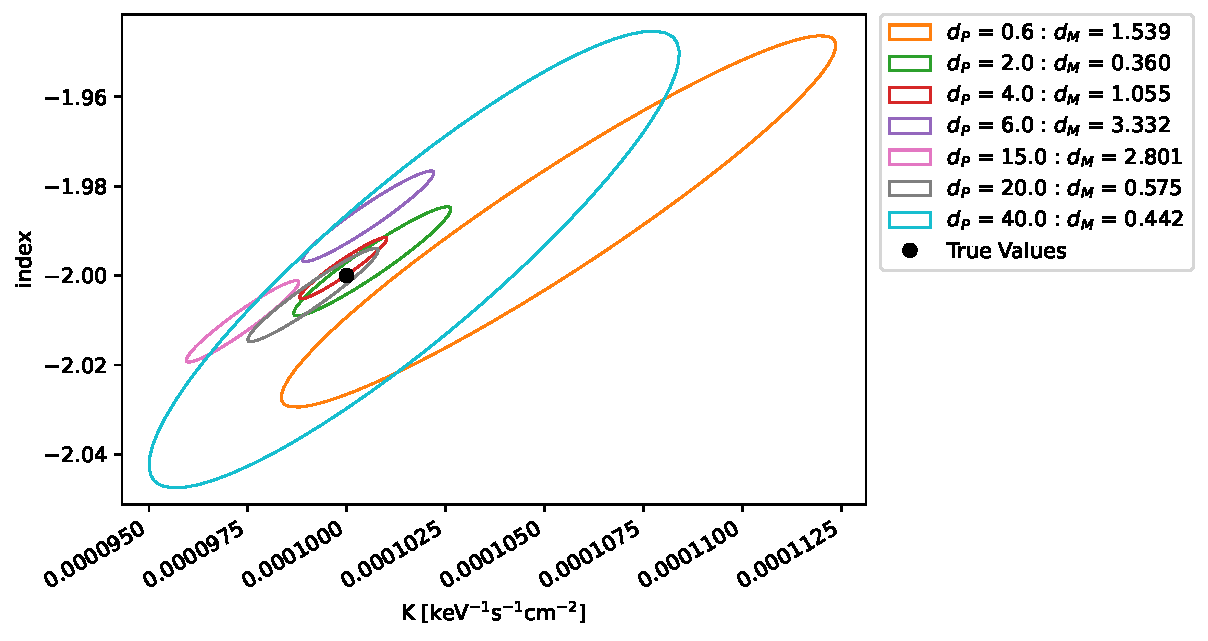
\includegraphics[width=\textwidth]{Images/Pure_Simulation/combined_plot_pointing_distances.pdf}
  \caption{Fit results for two SCWs with different angular distances $d_p$ (in degrees) between them. The center between the two SCWs is always orientated directly towards the source.}
  \label{fig pointing distances}
\end{figure}

A very important parameter when conducting these fits is knowing the optimal angular distance between SCWs in clusters, as shown in figure \ref{fig pointing distances}. Pointings with distances between 2 and 20 degrees all produced good results. Any angular distance outside of those values should be avoided. The very best result (with the smallest uncertainty) was attained for an angular distance of 4$^\circ$.

For this simulation and the next one the count spectrum was not simulated using the SCWs of revolution 0374 as a baseline, since custom orientations are required. Instead one cluster of 2 SCWs with custom orientations are used.


\subsection{Angular Distance between Source and Cluster}

\begin{figure}[h]
  \centering
  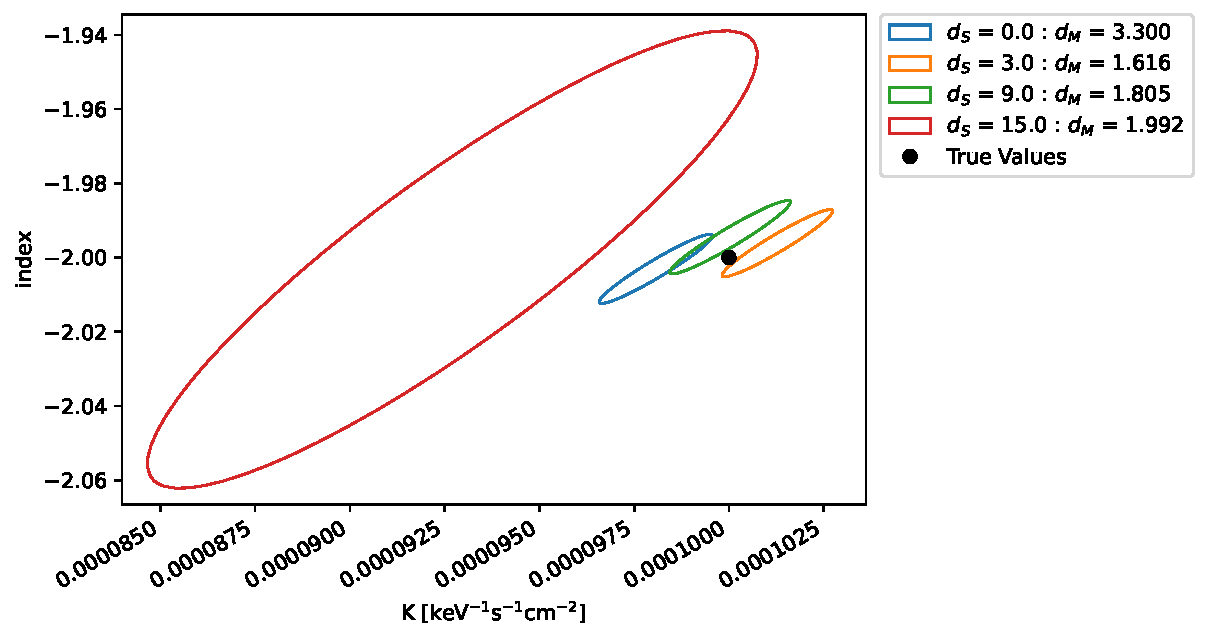
\includegraphics[width=\textwidth]{Images/Pure_Simulation/combined_plot_source_distances.pdf}
  \caption{Two SCWs with an angular distance of $4^\circ$ between them are clustered, and then rotated so that the center between them is $d_S$ degrees away from the source. The fit results for different results are shown.}
  \label{fig source distance}
\end{figure}

A similar yet equally important parameter for the SCW clustering algorithm is the maximum angular distance between pointings and the source. This is explored in figure \ref{fig source distance}. Anything within 9 degrees of the source provides equally good results, but as the distance approaches the edge SPIs $16^\circ$ field of view, the fit precision drastically worsens. 


\subsection{Cluster Size}

\begin{figure}[h]
  \centering
  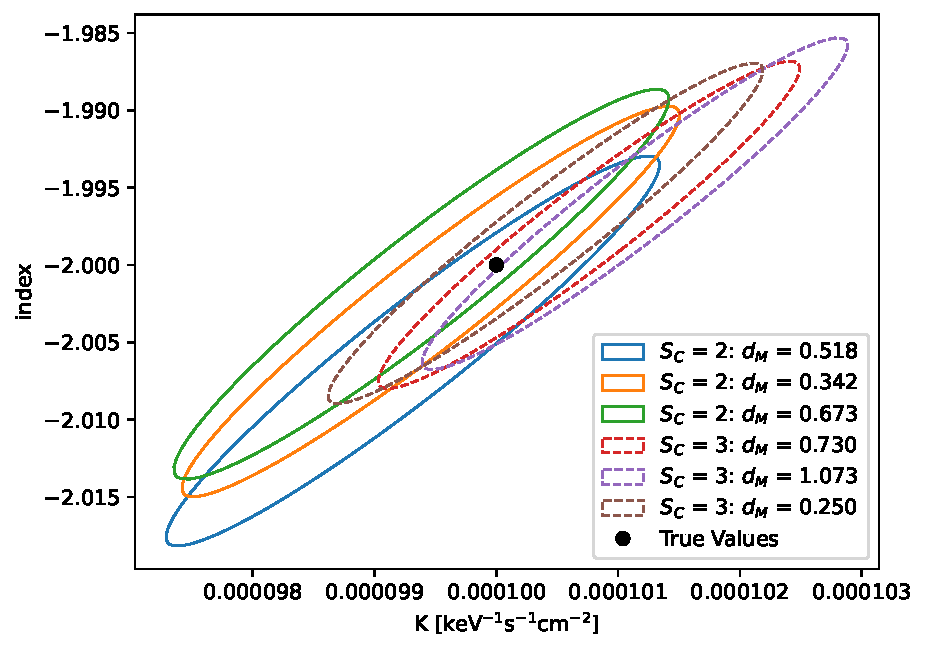
\includegraphics[width=0.7\textwidth]{Images/Pure_Simulation/combined_plots_cluster_size.pdf}
  \caption{The same dataset fitted repeatedly using clusters sizes $S_C$ of two and three.}
  \label{fig cluster size}
\end{figure}

So far we have only been using SCW clusters of size two ($S_C=2$) in the fits. Figure \ref{fig cluster size} compares fits using cluster size $S_C=2$ to $S_C=3$. Although the difference is not large, we do see a consistent improvement in both the distance from the true values and the uncertainty size of the fit parameters. Even larger clusters may accentuate this improvement even further. However, in practical applications larger cluster sizes also have downsides. For one, calculating the maximum likelihood background value becomes more complex, and secondly, the the assumption of a constant background count-rate within SCW clusters may become harder to fulfill, since larger cluster sizes necessarily mean larger temporal and spatial differences in the SCWs of the clusters.

\subsection{Fitting the Source Position}

\begin{figure}[h]
  \centering
  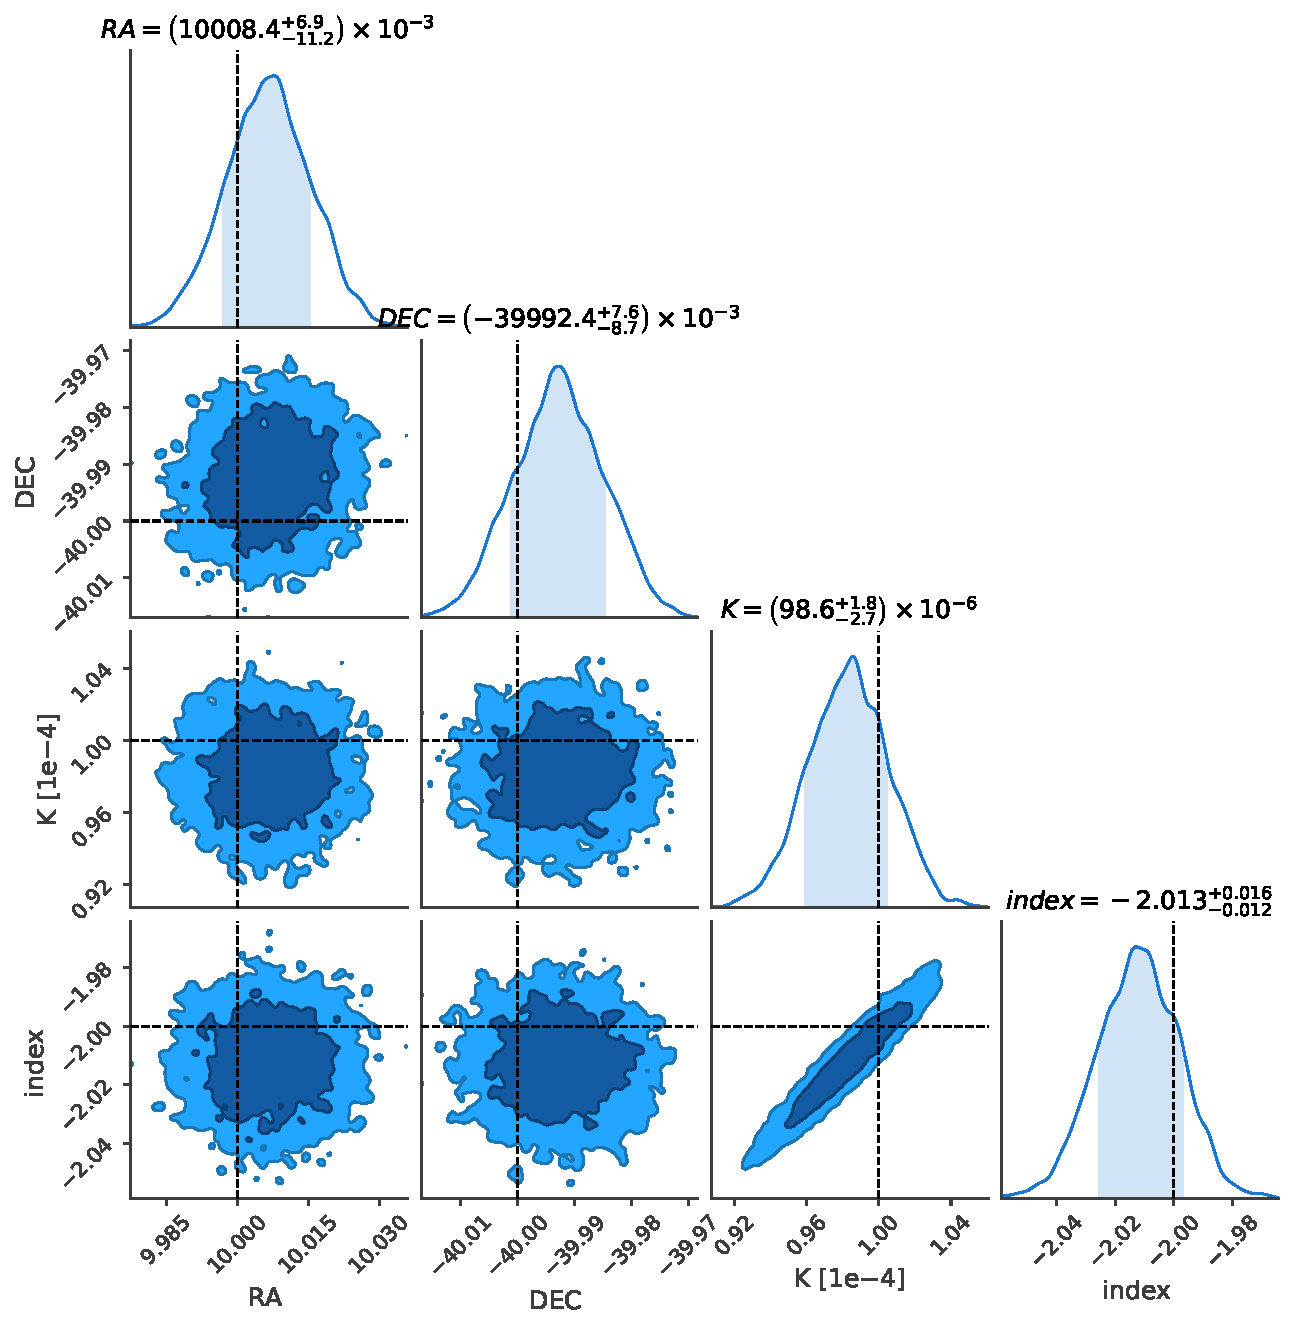
\includegraphics[width=\textwidth]{Images/Pure_Simulation/source_position.pdf}
  \caption{The posterior parameter distribution when fitting the source position along with spectral parameters. The dashed black lines indicate the true values.}
  \label{fig pos fit}
\end{figure}

Naturally we are not restricted to fitting spectral parameters of sources. The source position, for example, can also be included as parameters in the fit. The resulting posterior distributions of such a fit are shown in figure \ref{fig pos fit}. The results show a high degree of accuracy and precision, with all parameters within one standard deviation.


\section{Mixed Simulation and Spimodfit Comparison}




Having tested how well the PySPI fitting procedure works for purely simulated data where we know that the fundamental assumption of constant background rates is fulfilled, we may now move on to test how well the fit performs on mixed simulations, where the background counts are entirely real but the source spectrum remains simulated. This allows us to get a better understanding of how well the method works for realistic conditions but retain the advantage of knowing the true source model parameters in every fit. Additionally, this dataset is suitable to be fitted using Spimodfit due to it using real background counts, which the spimodfit background model is designed for. The procedure for using Spimodfit is described in appendix \ref{smf procedure}.

Before any fits can be conducted, a count spectrum needs to be created first. This can be done in almost the exact same steps as the purely simulated count spectrum form section \ref{sec: pure sim}, except step \ref{step pure sim back}, where we duplicate the counts from one SCW onto all other SCWs, is skipped entirely. This way the entire count spectrum from this revolution is used as background, and the simulated source counts are added on-top. Naturally, the choice of revolution is much more important here, since any sources in SPIs field of view will not be considered in the source model and hence invalidate the assumption of constant background rates within clusters. Revolution 0374 is used for this purpose, as it allows us to place our simulated source at the equatorial coordinates $RA=10^\circ, DEC=-40^\circ$, where no bright sources exist within SPIs field of view.

When fitting data using Spimodfit, a background model is created. This background model can be accessed (see section \ref{spimodfit bkg}) and provides us with another option for generating a count spectrum, as the simulated source counts can be added to the background counts from the spimodfit model.

\begin{figure}[h]
  \centering
  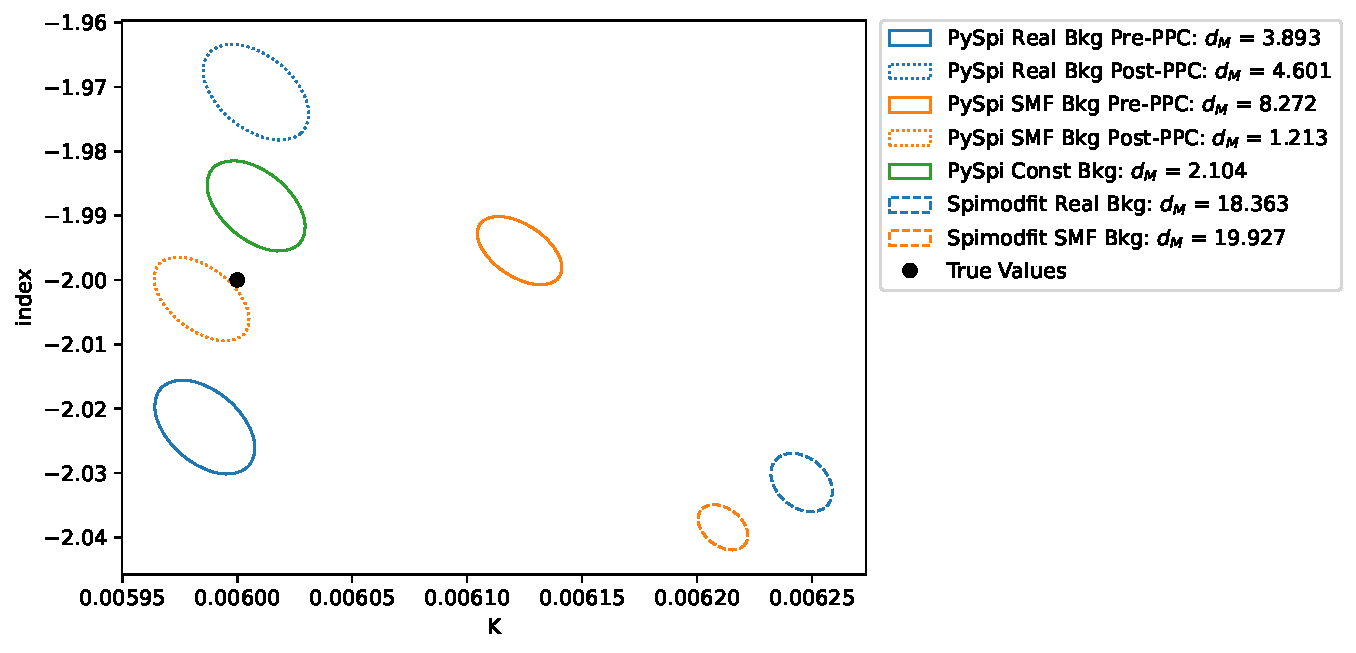
\includegraphics[width=\textwidth]{Images/SMF_Comparison/spimodfit_comparison_combined_plot.pdf}
  \caption{Fit results }
  \label{fig smf comparison}
\end{figure}

Both of these count spectra (real background counts and spimodfit background model counts) were fitted using PySPI and Spimodfit, the results of which are illustrated in figure \ref{fig smf comparison}. For further comparison purposes, a PySPI fit using the constant background counts (exactly as in section \ref{sec: pure sim}). The PySPI fits all perform comparably well. Perhaps the real background fit does worst, but this could just as well be a statistical fluctuation. Interestingly, the Spimodfit fits deliver consistently worse results, being almost 20 standard deviations away from the true values. Very curious is how using the Spimodfit fit using the Spimodfit background model as background counts in the data spectrum seems to make little difference in the fit quality. One would expect Spimodfit to do very well here, since its background model matches the background in the data perfectly.

All of these fits use an energy range of 30-81.5keV. The Spimodfit background model in particular is known to perform worse below 30keV, and it is possible that the SPI response function is not as accurate at the very edge of its energy range as well.





\section{Posterior Predictive Check (PPC) and Background Analysis} \label{sec:PPC Back}
Unusual solar activity, sources not included in the source model, and activation of satellite material from cosmic particles are just a few of the long list of causes may lead to errors in fit of SPI data. This is why Posterior Predictive Checks (PPCs) are a vitally important tool to analyze how well the results of fit actually match the data.

\subsection{PPCs: Theory}

\subsubsection{General Procedure} \label{PPC general}

A PPC is usually conducted in the following way:

\begin{enumerate}
    \item Fit the data to some model, so that a distribution for the posterior is produced.
    \item \label{Posterior sample} Randomly sample from the posterior.
    \item \label{ppc calc count rates} Using the IRF and the model described by the sampled posterior parameters, calculate the expected count rates in every energy bin of every detector of every SCW.
    \item \label{ppc poisson sample} Taking into consideration the lifetime of each detector in every SCW, draw a sample from the Poisson distribution that describes the measured counts in each bin.
    \item Repeat from step \ref{Posterior sample} until a sufficiently detailed distribution of expected counts for every bin is achieved.
\end{enumerate}

This PPC count distribution can the be used in a variety of ways, such as simply plotting the distribution of expected counts next the actually measured counts. Perhaps one of the most useful applications is the Cumulative Distribution Function (CDF), where one sorts the PPC count distribution of each bin according to size, and the finds the percentile in which the number actually measured counts falls. If the model described using the posterior values perfectly matches reality one would expect values evenly distributed between 0 and 1, whereas if the model is not a good representation of reality the distribution will not be even. 

In the context of PySPI it makes sense to organize these CDF values into a histogram for every SCW used in the fit. This way individual SCWs for which the model does not match the measured data can be identified and excluded from a repeated fit with hopefully better results. Experience has shown that "bad" SCWs often occur at the beginning or end of INTEGRAL revolutions, which is when SPI approaches its perigee and thus has the highest number of background events due to activation from cosmic particles. 

\subsubsection{PySPI Application}
As an attentive reader may have already identified, there is a problem with using the procedure previously described in section \ref{PPC general} for PySPI: the model used the fit (see section \ref{General Procedure}) is purely a source model, i.e. it tells us nothing about the background count rates. This is a problem because it means we cannot calculate the expected count rates in step \ref{ppc calc count rates} of section \ref{PPC general} without being able to describe the background.

The only way to circumvent this problem is with the same approach used in section \ref{General Procedure} of the actual fit. After having calculated the expected source count rates for a sample of the posterior we can use the actually measured counts to calculate the maximum likelihood background count rates and continue our analysis with it.

However, there is a drawback to this solution: in step \ref{ppc poisson sample} of section \ref{PPC general} we can no longer use a simple Poisson distribution to sample expected measured counts from the calculated count rates. This is because we have introduced a bias into our expected count rates by using the actually measured counts in the calculation. For example, if some energy bin has measured a statistically large number of counts (in accordance to the Poisson distribution of the true count rates), then the maximum likelihood background calculated using the actually measured counts will naturally increase with the actually measured counts. This way any statistical outliers are significantly dampened, thus defeating the purpose of conducting the PPC analysis to begin with.

To quantify this bias we will have to do some math. The following equations are applicable to every energy bin for every detector in every SCW cluster. As in section \ref{General Procedure} we will focus on clusters of size 2, although the process is analogous for larger cluster sizes.

For every bin and every SCW there exists a true source count rate $s_1$ and $s_2$ as well as a true background count rate $b$. The source count rates vary between the SCWs of one cluster, whereas the background count rate is constant. If $t_1$ and $t_2$ are the lifetimes of the SCWs, the actually measured counts $b_{1m}, b_{2m}, s_{1m}$ and $s_{2m}$ from the respective sources will be Poisson distributed

\begin{align*}
    B_{1m} &= P(bt_1) \\
    B_{2m} &= P(bt_2) \\
    S_{1m} &= P(s_1t_1) \\
    S_{2m} &= P(s_2t_2)
\end{align*}

so that the total number of measured counts $C_{1m}$ and $C_{2m}$ are simply

\begin{align*}
    C_{1m} &= B_{1m} + S_{1m} \\
    C_{2m} &= B_{2m} + S_{2m}.
\end{align*}

Arriving at an equation for the distributions $C_{1m}$ and $C_{2m}$ is our goal for the PPC analysis. We may assume that true source count rates $s_1$ and $s_2$ equal those predicted by our source model from the posterior samples, since testing that assumption is the whole point of doing the PPC analysis to begin with. The true background count rate $b$, however, remains unknown to us. Instead we can only calculate the maximum likelihood background $b_M$, as described previously. In order to be able to draw samples from the probability distributions $C_{1m}$ and $C_{2m}$ we must relate relate the distributions of the quantities that we do know ($s_1, s_2, t_1, t_2, b_M$) to those that we wish to know ($C_{1m}, C_{2m}$ and therefore $B_{1m}, B_{2m}, S_{1m}, S_{2m}$):

\begin{align*}
    B_{d1} &= B_{1m} - b_Mt_1 \\
    B_{d2} &= B_{2m} - b_Mt_2 \\
    S_{d1} &= S_{1m} - s_1t_1 \\
    S_{d2} &= S_{2m} - s_2t_2.
\end{align*}

$B_{d1}$ and $B_{d2}$ tell us the difference between quantities we have readily available ($b_Mt_1$ and $b_Mt_2$) to those directly necessary in the PPC analysis ($B_{1m}$ and $B_{2m}$). This means that if we calculate their variances and approximate the resulting distribution as normal we can directly draw random samples according to the distribution of $B_{1m}$ and $B_{2m}$, without having to know the true background rate $b$. Furthermore, we also have to consider that the distribution of $b_M$, which we utilize in $B_{d1}$ and $B_{d2}$, is correlated with the distribution $S_{1m}$ and $S_{2m}$. Hence, we not only have to calculate the variances of $B_{d1}$ and $B_{d2}$, but also the covariances of $B_{d1}$ with $S_{d1}$ and $B_{d2}$ with $S_{d2}$, respectively. To draw a random sample from $B_{1m}$, $S_{1m}$, $B_{2m}$ and $S_{2m}$we thus sample from a multivariate normal with mean $\mu$ and covariance matrix $cov$:

\begin{align}
    \mu_1 &= \begin{pmatrix}
        b_Mt_1 \\ s_1t_1
    \end{pmatrix} \\
    \mu_2 &= \begin{pmatrix}
      b_Mt_2 \\ s_2t_2
  \end{pmatrix} 
\end{align}
\begin{align}
    cov_1 &= \begin{bmatrix}
        variance(B_{d1}) & covariance(B_{d1}, S_{d1})\\ covariance(B_{d1}, S_{d1}) & variance(S_{d1})
    \end{bmatrix} \\
    cov_2 &= \begin{bmatrix}
      variance(B_{d2}) & covariance(B_{d2}, S_{d2})\\ covariance(B_{d2}, S_{d2}) & variance(S_{d2})
  \end{bmatrix}
\end{align}
Hence: 
\begin{align}
    \begin{pmatrix}
        B_{1m} \\ S_{1m}
    \end{pmatrix}
    &\sim \mathcal{N}(\mu_1, cov_1)\\
    \begin{pmatrix}
      B_{2m} \\ S_{2m}
  \end{pmatrix}
  &\sim \mathcal{N}(\mu_2, cov_2)
\end{align}
This works because the expected value of the maximum likelihood background rate is equal to the true background rate: $E(b_M) = b$. It is worth noting that approximating the distribution shapes as normal should have negligible impact as long as the number of counts per bin are sufficiently large.

Now that we have understood the motivation, the tricky part is actually calculating these variances. Considering the already complicated distribution of the maximum likelihood background (equation \ref{eq: max lik back})

\begin{equation*}
  b_M = \frac{1}{2} \left[ \frac{C_t}{t_t} - s_t + \sqrt{\left( \frac{C_t}{t_t} - s_t\right)^2 + 4 \left( \frac{C_1s_2+C_2s_1}{t_t}-s_1s_2\right)}\right]
\end{equation*}

where $C_1$ and $C_2$ are Poisson distributions, solving for the covariance matrices $cov_1$ and $cov_2$ analytically seems nearly impossible.


\subsection{PPCs: PySPI Implementation}

\subsection{Background Analysis}

\begin{figure}[h]
  \centering
  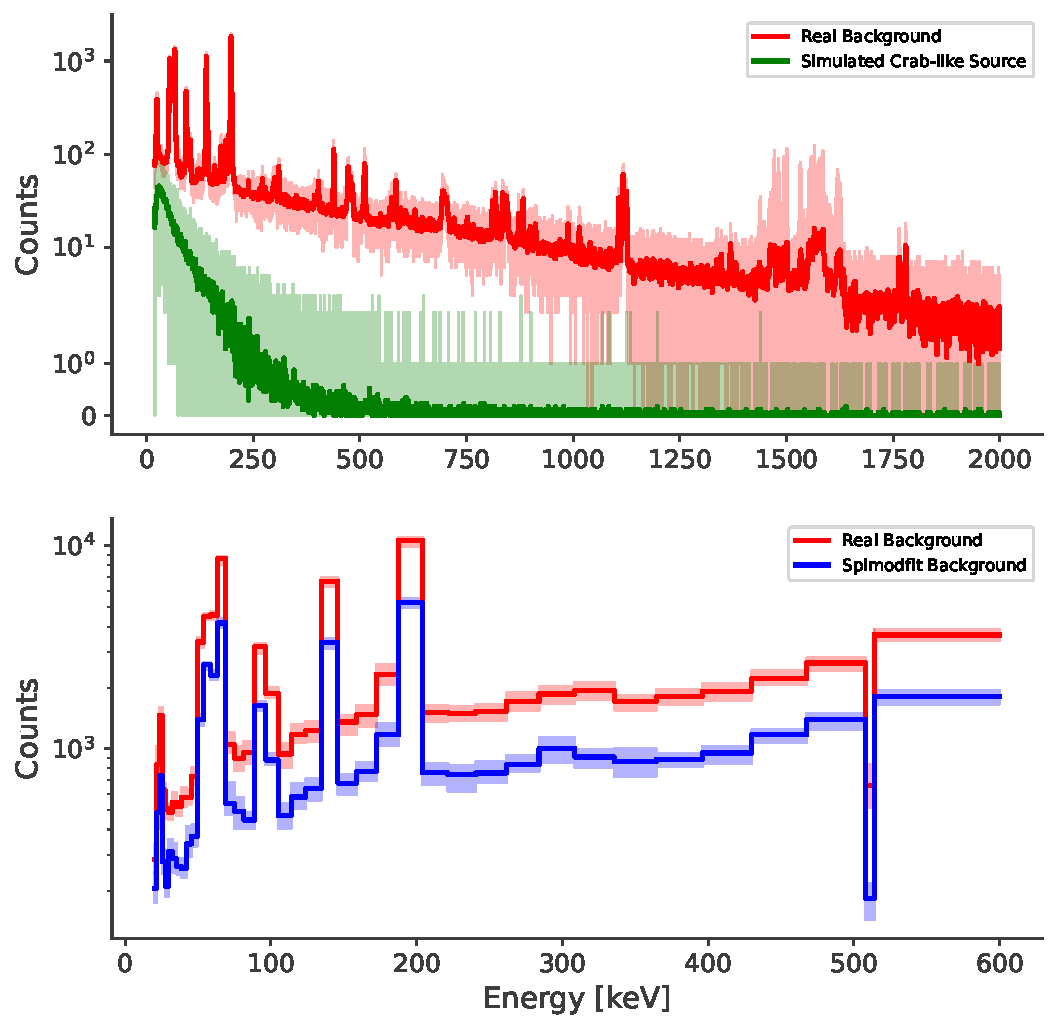
\includegraphics[width=\textwidth]{Images/PPC_and_Background_Analysis/background_spectrum.pdf}
  \caption{}
  \label{fig back spec}
\end{figure}


\appendix
\chapter{List of Source Models}

\subsection*{Powerlaw}

\begin{equation} \label{powerlaw}
  f(x) = K \frac{x}{piv}^{index}
\end{equation}

\begin{itemize}
  \item $x$: input energy [keV]
  \item $K$: differnetial flux at the pivot value, i.e. normalization [$\text{keV}^{-1}\text{s}^{-1}\text{cm}^{-2}$]
  \item $piv$: energy for which $K$ gives the normalized flux [keV]
  \item $index$: index of the powerlaw
\end{itemize}

\subsection*{Broken Powerlaw}
\begin{equation}
  f(x)= K~\begin{cases}\left( \frac{x}{x_{b}} \right)^{\alpha} & x < x_{b} \\ \left( \frac{x}{x_{b}} \right)^{\beta} & x \ge x_{b} \end{cases}
\end{equation}


\begin{itemize}
  \item $x$: input energy [keV]
  \item $K$: differnetial flux at the break energy $x_b$, i.e. normalization [$\text{keV}^{-1}\text{s}^{-1}\text{cm}^{-2}$]
  \item $\alpha$: powerlaw index for the low-energy half
  \item $\beta$: powerlaw index for the high-energy half
  \item $x_b$: break energy at which the broken powerlaw changes index [keV]
\end{itemize}

\subsection*{Smoothly Broken Powerlaw}

\begin{equation}
  f(x) = K \left( \frac{x}{x_b} \right)^{-\alpha}\left( \frac{1}{2} \left[ 1 + \left( \frac{x}{x_b}\right)^{1/\Delta} \right]\right)^{(\alpha - \beta)\Delta}
\end{equation}

\begin{itemize}
  \item $x$: input energy [keV]
  \item $K$: differnetial flux at the break energy, i.e. normalization [$\text{keV}^{-1}\text{s}^{-1}\text{cm}^{-2}$]
  \item $x_b$: The break energy at which the function is in-between powerlaw indices [keV]
  \item $\alpha$: low-energy powerlaw index
  \item $\beta$: high-energy powerlaw index
  \item $\Delta$: Smoothness parameter or break scale
\end{itemize}
Note: in practice this function was implemented slightly differently, so that the normalization $K$ describes the normalization at the pivot energy $piv$ instead of the break energy $x_b$

\subsection*{Band Function}
\begin{equation}
  f(x)= K~\begin{cases}\left( \frac{x}{piv} \right)^{\alpha}\text{exp}(-\frac{x}{x_p}) & x < x_{p}(\alpha - \beta) \\ \left( \frac{x}{piv} \right)^{\beta} \left[ \frac{(\alpha - \beta)x_p}{piv}\right]^{\alpha - \beta} \text{exp}(-(\alpha - \beta))& x \ge x_{p}(\alpha - \beta) \end{cases}
\end{equation}

\begin{itemize}
  \item $x$: input energy [keV]
  \item $K$: differnetial flux at the pivot energy, i.e. normalization [$\text{keV}^{-1}\text{s}^{-1}\text{cm}^{-2}$]
  \item $x_p$: characteristic energy of the band function [keV] 
  \item $\alpha$: low-energy powerlaw index
  \item $\beta$: high-energy powerlaw index
  \item $piv$: pivot energy at which the function is normalized [keV]
\end{itemize}

\chapter{Science Window Clustering Algorithm}
\label{Clustering Algorithm}
\section{Clustering Conditions} \label{list:conditions}
The fundamental idea of this project is the following: the SPI background event rates per detector per energy bin
is assumed to be constant between sufficiently close (in terms of time and orientation) pointings, and can thus be
determined analytically for bunches of several pointings via maximum likelihood calculations. This finally allows us to
apply Bayesian inference fits to determine source parameters. Since these fits are done on each cluster of pointings,
it is pivotal to write an algorithm that clusters a list of INTEGRAL pointings under the following conditions:
\begin{itemize}
    \item The angular distance between pointing orientations should not exceed a predetermined value within each
    cluster.
    \item The angular distance between pointing orientations should be higher than a predetermined value within each
    cluster. Many successive INTEGRAL pointings have nearly identical sky orientations, for which the coded mask
    produces nearly identical patterns; meaning that the above described method of eliminating the background parameter
    in the fits would not work. Hence a minimum angular distance within each cluster is necessary.
    \item The temporal distance between pointings should not exceed a predetermined value within each cluster.
    \item The number number of pointings in each cluster should be within some predetermined range of cluster sizes.
    Depending on the given list of pointings, clusters with fewer pointings than the preferred range may be
    unavoidable, but clusters with more pointings than the preferred range can definitely be avoided. A simple
    mechanism to encourage this is to minimize the total number of clusters, while never exceeding the maximum cluster
    size.
    \item The pointings should be as close as possible in order to justify the assumption that background rates are
    constant. Hence the average effective distance (composed of temporal and angular distance) between pointings should
    be minimized.
\end{itemize}


\section{Clustering Algorithm}
Clustering points in space together is a common problem in computer science, hence many sophisticated algorithms exist
to do so. However, the above listed conditions are rather unique, so an established clustering
algorithm that satisfies them was not found. The common sentiment for clustering algorithms is that there is no such thing as
the perfect clustering algorithm; instead the performance of the algorithm depends on how well it is suited to the type
of distributions found in the data. In our data, the pointings are distributed in three-dimensional space (one time and
two angular coordinates). However, they are not distributed randomly; instead the sky coordinates of INTEGRAL are
adjusted slowly as time progresses. Hence the data are distributed along a line through the time dimension, rather than
randomly distributed in the 3D space. With that in mind, the following clustering algorithm was developed:

\begin{enumerate}
    \item Given some list of pointings looking at an astronomical object, it is quite likely that INTEGRAL spends some
    time looking in the general direction, and then spends a lot of time looking at entirely different sections of the
    sky before returning to the astronomical object. Pointings with large temporal distances will never be clustered
    together, so the run-time of the algorithm can be reduced significantly by splitting the entire query of pointings
    into smaller, disconnected regions, so that the effective distance between any two pointings from different regions
    is larger than the predetermined maximum effective distance. However, in order to split the pointings into
    disconnected regions, the effective distance between any pair of pointings needs to be calculated. Given N
    pointings in our query, this requires computing an N by N matrix, which is computationally very expensive for large
    N. To improve this, the pointings are first split into preliminary regions, such that the temporal distance between
    any two temporally successive pointings in a preliminary region does not exceed the maximum effective distance.
    \item Now that we have reduced our large query into several smaller preliminary regions, we can compute the
    distance matrix for each preliminary region. Hence we have computed the distance matrix for any pair of pointings,
    except that we have only actually computed the distance for any relevant pair of pointings, and setting the value
    for pointings in different preliminary regions to some value higher than the maximum effective distance.
    \item While our preliminary regions are a good start, it is entirely possible that these are composed of several
    actual regions; i.e. that a preliminary region contains several regions of entirely disconnected pointings, where
    the effective distance between any pair of pointings from different regions is larger than the maximum effective
    distance. Since we have already computed the distance matrix for pointings within preliminary regions, we can use
    the following algorithm to split these into actual regions:
    \begin{enumerate}
        \item \label{itm: region1} Start with some point in the preliminary region, and assign it to a new region while
        removing it from the preliminary region.
        \item \label{itm: region2} Iterate through the preliminary region, and add any point with a distance smaller than the
        effective distance to the region, and remove said point from the preliminary region.
        \item Repeat the step \ref{itm: region2} for every pointing added to the region in the previous step.
        \item \label{itm: region4} If there are no more pointings to add to the region, repeat from step \ref{itm:
        region1} until the preliminary region is empty.
        \item Repeat steps \ref{itm: region1} to \ref{itm: region4} for all preliminary clusters.
    \end{enumerate}
    \item Now that have split the query into regions, we can cluster each region independently. This is done using the
    following algorithm:
    \begin{enumerate}
        \item First we need create an initial clustering, for which we can take advantage of the fact the the pointings
        are distributed along a temporal line in the 3D parameter space by iterating of the pointings in each regions
        according to the start date:
        \begin{enumerate}
            \item \label{itm: initial clustering 1}Create a cluster from the first un-clustered pointing.
            \item \label{itm: initial clustering 2} Iterate over some predetermined number of temporally successive
            pointings:
            \begin{enumerate}
                \item If the pointing can be added to the cluster without breaking the conditions listed in section
                \ref{list:conditions}, add it to the cluster and repeat from step \ref{itm: initial clustering 2}. If
                not, continue the iteration.
                \item When the iteration is finished or the cluster has reached is maximum size, continue from
                \ref{itm: initial clustering 1}.
            \end{enumerate}
        \end{enumerate}
        \item \label{itm: improvement1} While the initial clustering usually produces good results, there is no reason to assume that it is
        anywhere near optimal. For this reason we attempt an improvement on this clustering in the following way:
        \begin{enumerate}
            \item Randomly choose a sub-optimal cluster, weighted by cluster size. This is any cluster with less
            pointings than a predetermined number.
            \item Randomly choose a close sub-optimal cluster, weighted by distance from the first cluster and size. A
            second parameter is used to determine the maximum size of this cluster.
            \item Connect these two sub-optimal clusters through a path of clusters in the following way:
            \begin{enumerate}
                \item \label{itm: clustering path1}Find the pair of pointings with the least distance in the two clusters.
                \item Find the the pointings closest to the first of the two above pointings, that are not already part
                of the cluster path. Weigh these using their distance to the pointing, and by the angle between the
                vector connecting the first pointing to the target pointing, and the vector connecting the first
                pointing to the observed pointing. Randomly choose a pointing based on their weights.
                \item If the chosen pointing is in the target cluster, the path is complete. If not, repeat from step
                \ref{itm: clustering path1} using the cluster from the newly selected pointing as the first cluster.
            \end{enumerate}
            \item We will now re-cluster all pointings part of the cluster path:
            \begin{enumerate}
                \item \label{itm: reclustering1} Randomly choose a non-clustered pointing on the cluster path, weighted
                by its average distance to all other points on the cluster path. This way, the outlier points, which
                are most likely to be left without good clusters are clustered first. Create a cluster with this point.
                \item \label{itm: reclustering2} Randomly choose a non-clustered neighboring pointing on the cluster
                path, weighted by its distance to the current cluster and the distance to all other points on the
                cluster path. If it satisfies the conditions from section \ref{list:conditions}, add it to the cluster.
                \item Repeat step \ref{itm: reclustering2} until no points can be added to the cluster. 
                \item Then repeat from step \ref{itm: reclustering1} until all points on the cluster path are
                clustered.
            \end{enumerate}
            \item Calculate a cost of the new and old clustering configuration. Fewer clusters are better, and the
            average distance of all clusters is used as a tie-breaker. Keep the new configuration if it is better,
            otherwise keep the old one.
        \end{enumerate}
        \item Repeat from step \ref{itm: improvement1} until the number of successive rejected improvements exceeds a
        predetermined value.
    \end{enumerate}
\end{enumerate}

\chapter{Spimodfit Procedure} \label{smf procedure}

Spimodfit (see section \ref{about smf}) is an excellent tool to be able to compare SPI data fits against. The procedure for using Spimodfit is described in the steps below. In general, the  \href{https://www-cms.mpe.mpg.de/gamma/instruments/integral/www/}{Spimodfit cookbook} \cite{SMF_Cookbook} was followed very closely. In this thesis only the SE Data was used by Spimodfit with an energy up to 600keV, although this entire energy range was not used due to the problem of spurious events, as explained in section \ref{sec spurious events}.

\section{Fitting the Crab Nebula} \label{Spimodfit crab steps}
The following procedure is used to fit the Crab Nebula:

\begin{enumerate}
    \item On the ga05us.mpe.mpg.de PC, head into the directory:
    
    \verb|/home/jmoeller/cookbook/SPI_cookbook/examples/Crab|

    \item \label{scw select} In the file \verb|spiselectscw.cookbook_dataset_02_0020-0600keV_SE.par| specify which revolution(s) is to be used via the \verb|fits_revolutions_list| and \verb|revolutions_cond_value| parameters. Run the script:
    
    \verb|./submit-spiselectscw_ga05us.sh cookbook_dataset_02_0020-0600keV_SE &|

    This selects relevant SCWs from chosen revolutions and prepares the necessary data files for the fit.

    \item \label{step background} In the file \verb|background_model_SE_02.pro| change the parameters \verb|spidir|, \verb|scw_file|, and \verb|bgdir| to point towards the correct directories in the newly created directory 
    
    \verb|cookbook_dataset_02_0020-0600keV_SE|. Run this script: 
    
    \verb|idl idl-startup.pro background_model_SE_02.pro|

    This creates the spimodfit background model for the relevant SCWs.

    \item \label{Source directory} In the file \verb|spimodfit.fit_Crab_SE_02.par| change the parameters 
    
    \verb|counts_input_file|, \verb|pointing_input_file|, \verb|ebounds_input_file|, \verb|deadtime-dol|, \verb|gti-dol|, 
    
    and \verb|background_input_file| to point to the correct directories. Furthermore, specify the source catalogue directory:
    
    \verb|source-cat-dol,s,h,"/home/jmoeller/cookbook/SPI_cookbook/cats/cat_crab.fits.gz"|

    Leave everything else untouched and run the script:

    \verb|./submit-spimodfit_v3.2_ga05us.sh fit_Crab_SE_02 clobber &|

    This fits the source to the data using the background model.

    \item \label{Spectrum file} Inside the directory \verb|fit_Crab_SE_02| run the script \verb|./spimodfit_rmfgen.csh|. Back in the previous directory, edit the parameters \verb|response_file| and \verb|spectrum_file_01| in the file 
    
    \verb|adjust4threeML_SE_02.pro| to point at the correct directories, and run the script:
    
    \verb|idl idl-startup.pro adjust4threeML_SE_02.pro|

    This makes some slight formatting adjustments so that they fitted source spectra are more convenient to use. 

    \item For convenience, transfer the files \verb|specra_Crab.fits| and \verb|spectral_response.rmf.fits| onto the local machine. Here the script found in
    
    \verb|/home/jmoeller/cookbook/SPI_cookbook/spectral_analysis/3ml_fit_Crab_SE.py|
    
    is used extract the fit parameters, where the source model and active measurements (i.e. energy range) can be changed as pleased.
\end{enumerate}


\section{Fitting other Sources}
If we want to fit another source (or multiple) instead of the Crab, the following changes are made to the previously described steps:

\begin{enumerate}
    \item Access the SPI source catalogue: \verb|/home/jmoeller/cookbook/SPI_cookbook/cats/spi_cat.fits.gz|
    \item Create a new file with only one (or more, depending on how many sources we want to fit) row from the source catalogue, representing one source. Edit the entries \verb|RA_OBJ|, \verb|DEC_OBJ|, and \verb|NAME| to the coordinates and name of the new source. Other entries in the row are not used and irrelevant for the fit.
    \item Place the new file in the same directory as the original catalogue.
    
    Now repeat steps from section \ref{Spimodfit crab steps} with the following differences:
    \item In step \ref{scw select} from section \ref{Spimodfit crab steps} also change the parameters 
    
    \verb|select_PtgX_masks_chi_list_1| and \verb|select_PtgX_masks_psi_list_1| 
    
    to the coordinates of the new source. Note that these are galactic coordinates.
    \item In step \ref{Source directory} from section \ref{Spimodfit crab steps} change \verb|source-cat-dol| to instead point to the new source file.
    \item The new spectrum output file will be names according to the new source name, which has to be reflected in the parameter \verb|spectrum_file_01| from step \ref{Spectrum file} in section \ref{Spimodfit crab steps}. Furthermore, if multiple sources are fitted simultaneously, analogously create a new parameter \verb|spectrum_file_02| for every source spectrum.
\end{enumerate}


\section{Fitting Custom Data}
If we want to use Spimodfit to fit our own custom data, for example for simulated sources, we can once again repeat the steps from section \ref{Spimodfit crab steps} with one difference. After step \ref{scw select} is completed the directory

\verb|/home/jmoeller/cookbook/SPI_cookbook/examples/Crab/cookbook_dataset_02_0020-0600keV_SE/spi|

is created, which includes the relevant data files to be used in the fit. Here we can edit \verb|evts_det_spec.fits.gz| to our custom data, which obviously has to take into consideration which SCW, detector, and energy bin each table entry corresponds to. 


\section{Spimodfit Background} \label{spimodfit bkg}
For every fit, Spimodfit creates a background model. After step \ref{step background} in section \ref{Spimodfit crab steps} is completed the directory

\verb|/home/jmoeller/cookbook/SPI_cookbook/examples/Crab/cookbook_dataset_02_0020-0600keV_SE/|\newline
\verb|spi/bg-e0020-0600|

is created, containing the files \verb|output_bgmodel-conti.fits.gz| and \verb|output_bgmodel-lines.fits.gz|. These contain the expected number of counts for each energy bin from each detector in each SCW. In order to obtain a usable background model one can add the count rates from the both files together and then Poisson distribute the result.

\nocite{*}
\printbibliography



\end{document}